\documentclass[sigconf]{styling/acmart}
%% NOTE that a single column version may required for 
%% submission and peer review. This can be done by changing
%% the \doucmentclass[...]{acmart} in this template to 
%% \documentclass[manuscript,screen]{acmart}
%% 
%% To ensure 100% compatibility, please check the white list of
%% approved LaTeX packages to be used with the Master Article Template at
%% https://www.acm.org/publications/taps/whitelist-of-latex-packages 
%% before creating your document. The white list page provides 
%% information on how to submit additional LaTeX packages for 
%% review and adoption.
%% Fonts used in the template cannot be substituted; margin 
%% adjustments are not allowed.

\usepackage{styling/additional_dependencies} % Bring in all the includes and Latex Utils

%%
%% \BibTeX command to typeset BibTeX logo in the docs
\AtBeginDocument{%
  \providecommand\BibTeX{{%
    \normalfont B\kern-0.5em{\scshape i\kern-0.25em b}\kern-0.8em\TeX}}}

\begin{document}
    % Everything prior to the main body of content

% Tell TexCount to ignore words in word count
%TC:ignore
% \pagenumbering{gobble} % Don't track page numbers prior to Table of Contents
% \thispagestyle{empty} % Remove Page Styling prior to Table of Contents
% \newgeometry{inner=0.2\textwidth,outer=0.2\textwidth}

%% Rights management information.  This information is sent to you
%% when you complete the rights form.  These commands have SAMPLE
%% values in them; it is your responsibility as an author to replace
%% the commands and values with those provided to you when you
%% complete the rights form.
\setcopyright{acmcopyright}
% \copyrightyear{2018}
% \acmYear{2018}
\acmDOI{XXXXXXX.XXXXXXX}

%% These commands are for a PROCEEDINGS abstract or paper.
\acmConference[Conference acronym 'XX]{}{N/A}{N/A}
%
%  Uncomment \acmBooktitle if th title of the proceedings is different
%  from ``Proceedings of ...''!
%
%\acmBooktitle{Woodstock '18: ACM Symposium on Neural Gaze Detection,
%  June 03--05, 2018, Woodstock, NY} 
% \acmPrice{}
% \acmISBN{}

% Setup title
\title{Distinguishing Between Head and Phone Gestures On a Smartphone With Front-Facing Camera and IMU}
% \renewcommand\maketitlehookb{\centering \Large }
\date{\today}
\author{James Whiffing} % Presume should also list supervisors here, but need to indicate?
% \authornote{}
\email{jw204@bath.ac.uk}
% \orcid{1234-5678-9012}
\affiliation{%
  \institution{University of Bath - Department of Computer Science}
%   \streetaddress{P.O. Box 1212}
  \city{Bath}
  \country{England}
%   \postcode{43017-6221}
}
%%
%% By default, the full list of authors will be used in the page
%% headers. Often, this list is too long, and will overlap
%% other information printed in the page headers. This command allows
%% the author to define a more concise list
%% of authors' names for this purpose.
\renewcommand{\shortauthors}{Whiffing, James}

%%
%% The abstract is a short summary of the work to be presented in the
%% article.
\begin{abstract}
  \tempnote{TODO}
\end{abstract}

%%
%% The code below is generated by the tool at http://dl.acm.org/ccs.cfm.
%% Please copy and paste the code instead of the example below.
%%
\begin{CCSXML}

\end{CCSXML}

% \ccsdesc[500]{Computer systems organization~Embedded systems}
% \ccsdesc[300]{Computer systems organization~Redundancy}
% \ccsdesc{Computer systems organization~Robotics}
% \ccsdesc[100]{Networks~Network reliability}

%%
%% Keywords. The author(s) should pick words that accurately describe
%% the work being presented. Separate the keywords with commas.
% \keywords{} % TODO

%% A "teaser" image appears between the author and affiliation
%% information and the body of the document, and typically spans the
%% page.
\begin{teaserfigure}
  \center
  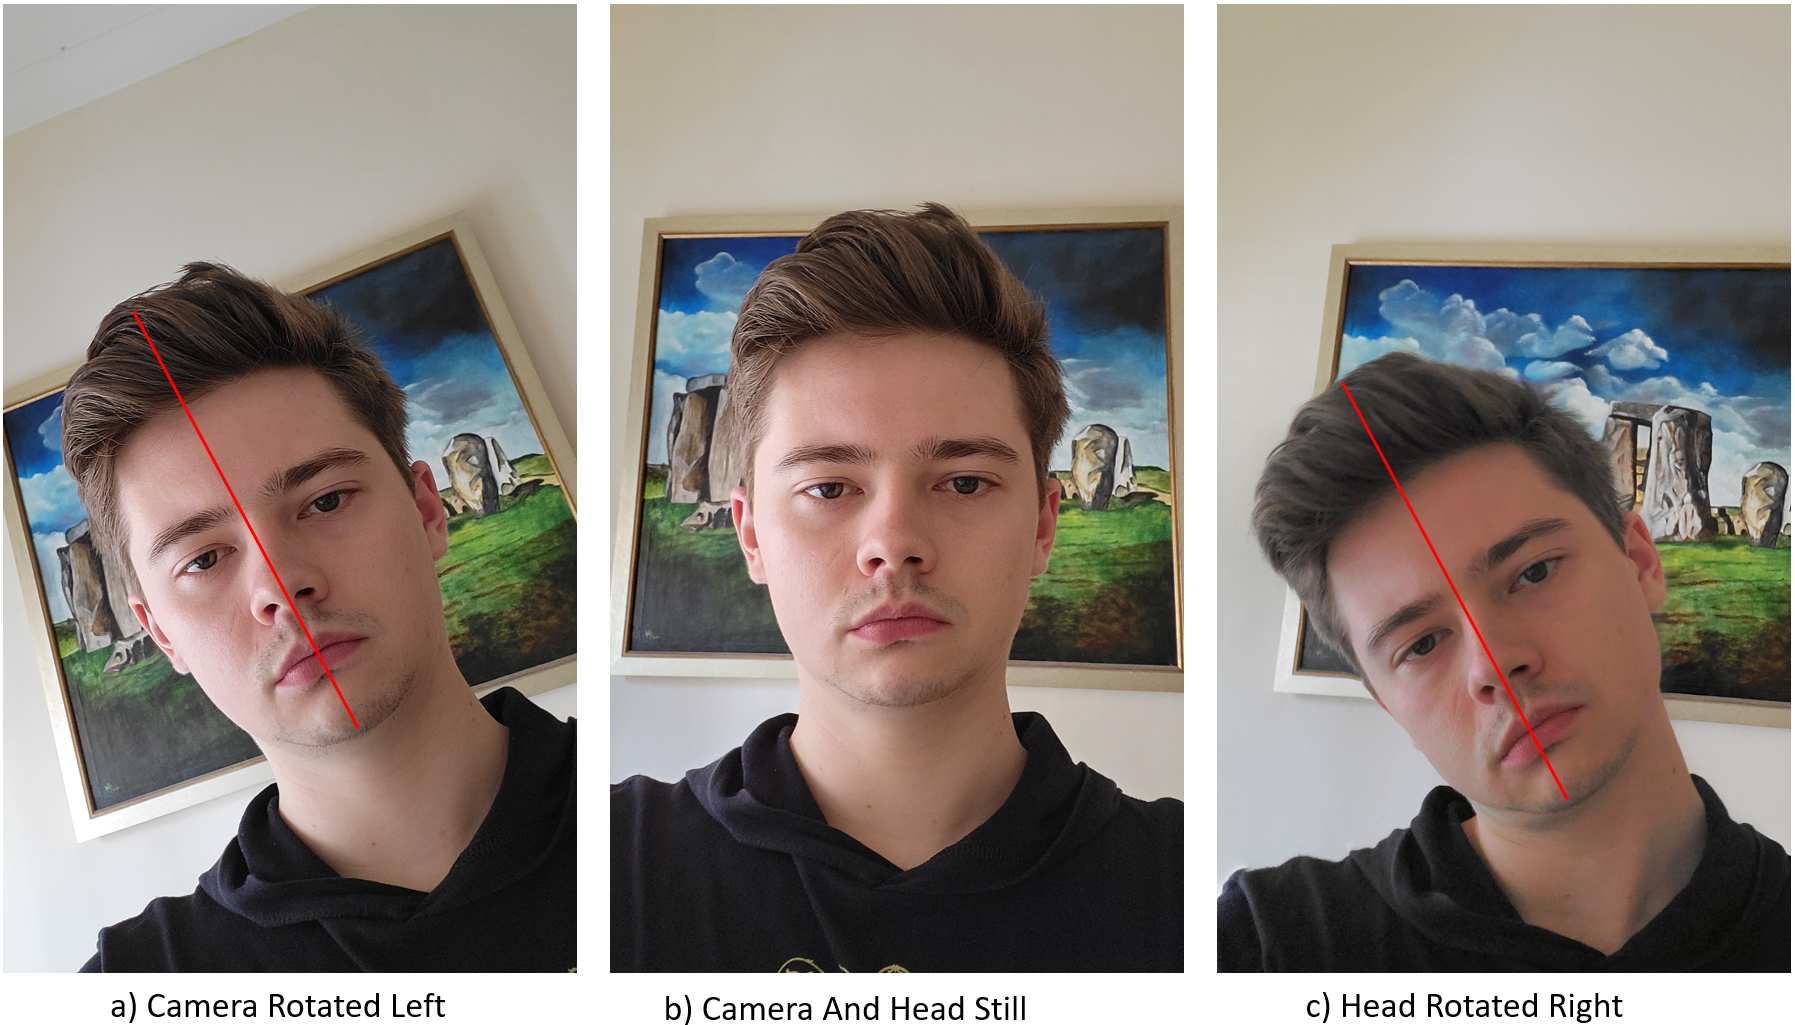
\includegraphics[width=0.65\textwidth]{figures/HeadOrientations.png}
  \caption{Demonstration of how changes in head or phone orientation can result in the same head orientation being observed by a smartphone's front-facing camera}
  \label{fig:teaser}
  \Description{Diagram showing how a the head pose observed by the front-facing camera of a mobile device, caused by the movement of the head, can be replicated by keeping the head still and instead moving the camera.}
\end{teaserfigure}

\maketitle
%% Content Lists %%

% \clearpage
% \restoregeometry
% \newpage

% \setcounter{page}{0}
% \pagenumbering{roman}
% \pagestyle{fancy}

% \tableofcontents
% \clearpage
% \newpage
% \addcontentsline{toc}{section}{\listfigurename}
% \listoffigures
% \clearpage
% \newpage
% \addcontentsline{toc}{section}{\listtablename}
% \listoftables
% \clearpage
% \newpage

% Tell TexCount to start counting words again
%TC:endignore

% Reset Page Styling and numbering for rest of doc
% \setcounter{page}{1}
% \pagenumbering{arabic}

    \section{Introduction} % 0.5 Pages
%% What 
% State of The World:
Touchscreens have been the primary interface with which users interact with modern smartphones, either through directly touching UI elements (such as buttons or an on-screen keyboard) or through the use of touch-gestures. 
Over recent years there has been a trend of smartphone touchscreens increasing in size\cite{xuesheng2018research}, which does not afford optimal reachability of the full screen for the thumb for interactions\cite{le2018fingers}. This reduces usability for one-handed interaction, which is a common mode of use\cite{hoober2013users}
\\\\
An emerging solution to this is to include head gestures as an additional mode of input, by tracking the head via the smartphone's front-facing camera\cite{gorodnichy2004nouse, deepateep2020facial, voelker2020headreach, roig2015face, hansen2006use, francone2011using}.
A problem with tracking something via a camera that can have a moving Point-of-View (PoV) is that changing the camera's PoV can \textit{look} like movement of the object being tracked.
For example, the user moving their phone to the left, will be treated the same as the user moving their head to the right, since the positioning and movement of the head from the front-facing camera's point of view will look the same, see \autoref{fig:teaser}.
Some papers knew of this issue and accept it as a feature\cite{hansen2006use}, others note it as a known fault to be aware of\cite{francone2011using, varona2008hands}, while others don't indicate whether this has been accounted for\cite{gorodnichy2004nouse, deepateep2020facial, voelker2020headreach,roig2015face}.
\\\\
% Research Question:
In this paper we look to propose a system that can distinguish between the head or smartphone being moved. In being able to differentiate the two, it should also be able to recognise gestures based on the smartphone movement.

% Solution/What We Did:
In order to develop a proof-of-concept, a data driven approach was taken.
As such a study was performed to collect data: image sequences from the front-facing camera of the smartphone, IMU data from the smartphone, and 3D positioning of the user's head and the smart device via a motion capture system (to provide a ground truth).

With the motion capture data being synced to the IMU data and images, a system could be trained to recognise several gestures and learn to distinguish between whether an observed gesture was due to the smartphone or the user's head moving.

% What was the system's performance? Did we succeed?
% How is the work to be extended?

    \section{Literature Review} % 2-3 Pages
In this section we will review existing literature to build an understanding of: the gestures we can expect to process, how they may be used and what they mean; Methods with which to obtain data pertaining to the pose of a head; and finally the means with which we can track movement and determine the gesture being performed.
% Types of Head Gestures (Pointing (Dietic & Manipulative) vs Semaphoric)
%   Since used by the systems mentioned in the intro, discuss these 3 types
%   Why would these types of gestures be used, what roles did they serve.
%   Examples of these gestures (with regards to systems referenced in intro)
% Probably a small section

% Head Tracking (From Smartphones)
% How track head, (Front facing camera, )
% Cascades, need face first, or one model (if using NN/ML solutions)
%   - IMU (From Head Mounted Displays and Head Mounted IMU)
%       - Will intend to use earbuds to collect IMU data of head, make footnote mentioning that this this was unfortunately not completed within this paper
%   - CNNs
%   - HAAR
%   - Alternatives (Feature extraction via histograms, etc)

% Head Gesture Recognition
% How did reviewed systems do this?
% Given data, how determine gesture performed, e.g. Dietic pointing (use raw data, e.g. calculate screen region/pointer position from data) vs Semaphoric/Manipulative classifying (given data, determine gesture performed)
%   - Derived
%   - Regression NN?
%   - RNN/LSTM (papers not specific to mobile phones)
%       - given a sequence, what class does it belong to?
%   - Markov Chain
%       - Given current state and new input, what is the new state?

% Merge last 2 sections into one?

\subsection{Gesture Classifications and Usage} % Types of Head Gesture
% Types of Head Gestures (Pointing (Dietic & Manipulative) vs Semaphoric)
%   Since used by the systems mentioned in the intro, discuss these 3 types
%   Why would these types of gestures be used, what roles did they serve.
%   Examples of these gestures (with regards to systems referenced in intro)
% Probably a small section

% Gesture classes and then discuss their examples / use-cases?
% Or
% Papers and examples, and then classification?

% Discuss why might want head gestures ?
%   - Any cases where these motions may be useful for SIIDs (Situationally Induced Impairments or Disabilities)?
% add more input options, not rely on using intuitive gestures that have since become system gestures (android navigation gestures) \cite{hueber2020headbang}

% Outline the types of gesture, and of those, which ones head gestures can b classified as.
% From example papers regarding head gesture control for mobile devices, look into 

Given our goal is to develop a means to distinguish head and phone gestures on smartphone devices, we first need to understand the gesture's we want to recognise and distinguish.
Here we will look at existing literature that outline the head and phone gestures you would expect to use while interfacing with a smartphone.
\\\\
% Mention classes defined > mention ignore 2 as unrelated to head-gestures > explain exemplars of each type > Summary suggesting multiple employed by each system?
% Mention classes defined and list > mention ignore 2 as unrelated to head-gestures > describe several exemplars and what style/s they fit into?
% Mention classes defined and list > mention ignore 2 as unrelated to head-gestures > describe how in our review of literature that we classify as pointing/cursor manipulation vs semaphoric (gesture maps to action)
%
% https://eprints.soton.ac.uk/261149/1/GestureTaxonomyJuly21.pdf
% Breakdown the relevant gestures
After a review of gestures utilised within Human Computer Interaction literature \citeauthor{karam2005taxonomy} define five distinct classes with which we can differentiate between types of gestures utilised by the systems proposed in the literature\cite{karam2005taxonomy}:
\begin{description}
    \item[Dietic] Gestures that involve pointing, and mapping this to either a specific object or location within the interface.
    \item[Manipulative] A gesture which indicates intent to manipulate some object.
    \item[Semaphoric] Gestures which map to a specific action or intent.
    \item[Gesticulative] Typically accompany speech, but not required to transfer meaning.
    \item[Language] A substitute to written or verbal language.
\end{description}

In our review of head/phone gesture systems we found that none utilised the Language or Gesticulative gesture styles, which is to be expected as we were focusing on gestures for control and interaction rather than for communication.
Of the 3 remaining gesture styles, we noted that systems rarely utilised a single gesture style. Either due to the gestures themselves being viewable as multiple gesture styles, being both semaphoric and manipulative, or by actively including different styles of gestures,such as pointing to a region, then using a sempahoric gesture to trigger an action.
% detail examples showing the gestures they decided upon, and why.
% example the types of gestures
% how might a phone gesture differ from head
% why might they look the same?
% yan2018headgesture, they explored existing head gestures (maybe focusing on those trackable via IMU over other methods?). Their study resulted in details shown in figure
\begin{figure}
    \centering
    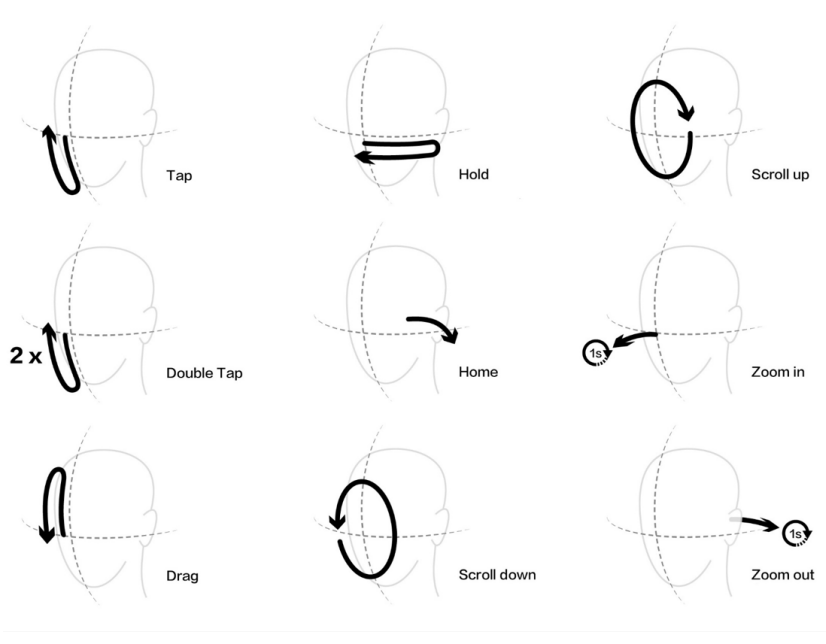
\includegraphics[width=0.5\textwidth]{figures/yan2018headgesture_fig2_proposed_gestures.png}
    \caption{\label{fig:yan2018headgesture_proposed_gestures} Proposed head gestures and their corresponding actions\cite{yan2018headgesture}.}
    \Description[9 diagrams depicting the gestures proposed by \citeauthor{yan2018headgesture}]{9 diagrams depicitng the path of the nose taken to perform each gesture proposed by \citeauthor{yan2018headgesture}.} % Expand on this
\end{figure}
\\\\
An example of this can be seen in the work of \citeauthor{yan2018headgesture}\cite{yan2018headgesture} who propose 9 head gestures (\autoref{fig:yan2018headgesture_proposed_gestures}), the majority of which are purely semaphoric, however several (such as scrolling, dragging, and zooming) could also be seen as manipulative through the mapped action physically moving the content on screen.
\citeauthor{yan2018headgesture} derived these gestures through a study wherein participants where asked to proposed a set of head gestures, without being given an associated action. These gestures were then collated manually into a set of 80 gestures, which were then effectively voted upon by the participants for their respective actions.
The gestures with the most votes for a given action were selected, with some minor adjustments to ensure there were no clashes between actions.

Another system that utilised multiple gestures was EyeMu\cite{kong2021eyemu}, which outline several gestures, that are performed by physically moving the smartphone, to extend user interaction when user is forced to interact with phone single handed.
As with \citeauthor{yan2018headgesture}'s gestures, most are semaphoric, but can be viewed as manipulative.
Some map to actual actions, e.g. flicking between items, others are less derivative and have less of a connection to the desired effect, e.g. moving phone closer/further from face to select an item / open a page.

% NOUSE
Two systems that were purely dietic are Nouse\cite{gorodnichy2004nouse} and a system developed by \citeauthor{varona2008hands}\cite{varona2008hands}, both of which maps the position of the user's nose in images from the front-facing camera to a location on the screen.
Neither system recognises sequences of motions of the head as gestures, other than recognising blinking and winking, which were recognised as an action to select what was under the cursor. 
You could also argue that these systems are also manipulative given they show a cursor and as such the head gestures are in an attempt to move the cursor to the relevant location.

% https://projet.liris.cnrs.fr/imagine/pub/proceedings/CVPR2012/data/papers/workshops/W01_05.pdf
\cite{lopez2012head} utilise a form of Manipulative gestures, wherein the pose of the head is used to either adjust the view of what is on screen, emulating a change in perspective, or by changing the UI (such as opening th ebookmarks bar while looking at a webpage)

% Head bang and reach
% Initially used to 

% Phone gestures
% https://dl.acm.org/doi/pdf/10.1145/3462244.3479938

\subsection{Head Feature Extraction and Localisation}
% Head Tracking (From Smartphones)
% How track head, (Front facing camera, )
% Cascades, need face first, or one model (if using NN/ML solutions)
%   - IMU (From Head Mounted Displays and Head Mounted IMU)
%       - Will intend to use earbuds to collect IMU data of head, make footnote mentioning that this this was unfortunately not completed within this paper
%   - CNNs
%   - HAAR
%   - Alternatives (Feature extraction via histograms, etc)
%   - Optical Flow

% Want to have headings, or just have paragraphs?
% TODO: Better intro
Before being able to distinguish between head and phone gestures, we first need to extract them. To start with we will be reviewing the methods in surrounding literature to extract relevant data required to track head gestures through the use of a smartphone.
%split this section into both feature extraction and tracking?


\subsubsection{HAAR Cascades / The Viola Jones Algorithm}\nl
(Viola Jones Algorithm\cite{viola2004robust})
% An aside on use to extract location of face, but no features
% Application of filters representing features found on common faces.
% Applied in a cascade, e.g. only check for next set of features if found large one.
% Used to reduce search space / and limit data that needs processing.

% Can be extended to also extract the location of features
% https://www.proquest.com/docview/1927472131?fromopenview=true&pq-origsite=gscholar
\cite{kim2017real} Utilise HAAR-like features with an Adaboost classifier to detect 4 features: left eye, right eye, nose-tip, and mouth.

Use Greyscale image, and use integral image (summed area table) to apply the features.
Determine head pitch and yaw (not roll).

% However typically used to narrow down the search space for subsequent logic
\cite{neto2012real} Also utilise HAAR-like features in a classifier, however they simply use this to identify the region of the image that contains a face, and then utilise a histogram of pixel intensity (amount of variation in a given slice of the image) to identify the eyes.
This is done once during calibration to then extract the eyes (left eye 30\% along the line, right is 70\%) and nose (if the eyes are $d$ far apart, the nose is $d*0.45$ below the midpoint between the eyes), assuming head is upright and user is facing camera.

A downside to the V-J algo is "Informal observation suggests that the face detector can detect faces that are tilted up to about ±15 degrees in plane and about ±45 degrees out of plane (toward a profile view). The detector becomes unreliable with more rotation than this."\cite{viola2004robust}

% Random forrest?

\subsubsection{Convolutional Neural Network (CNN)}\nl
% train model that extracts features that found in faces
% either predict: face exists, Region of image containing face, Derived features of face (size, rotation, landmarks, etc)

% Alternatives???
\cite{yan2021fast}

% Android MLkit for face detection?

% Some use HAAR cascades to narrow down region
% Some alo output similar to HAAR, e.g. bounding box
% Even open CV, which has had VIOLA-Jones algo built-in now recomends use of CNN (YUNET?) instead of their HAAR classifier

\subsubsection{Colour Segmentation}\nl
Either removing all colours that aren't within the defined colour space, to then perform additional processing, such as edge detection, or using histograms to find regions in the image of given colours to detect features?


\subsection{Phone Localisation and Tracking}
% We now have several methods we can refer to in order to determine the head gesture being performed by a user, however we now need to explore the final area in the related works: recognising phone gestures. 
During our review of related works we came across several means of localising a smartphone / tracking a smartphone's movement, each with varying degrees of feasibility.

The least reasonable methods do not bare reviewing due to unrealistic expectations of the population of smartphone users, such as the need for a Motion Capture (MoCap) system\cite{buschel2017investigating} or the use of a Head Mounted Display with a mounted tracking marker\cite{mohr2019trackcap}.
These may be suitable in specific environments, but are not reasonable in meeting our goal.
\\\\
A more reasonable set of methods involve localising the smartphone's position relative to its environment.
\tempnote{Picture of features used for camera tracking}\\
One method is 'camera tracking', wherein the movement of the camera is estimated through analysis of an image stream from the rear-facing camera. This is a technique common-place in VFX to recreate the path taken by a camera in 3D\cite{barber2016camera}, but has also been extended to use in Augmented Reality applications\cite{jiang2000camera}.
Unfortunately this isn't reasonable to use on current modern mobile phones as they don't all support the ability to capture images from multiple cameras (some via software, others due to hardware limitations). As such we will not be able to utilise the rear camera as the front-camera will be required to track the user's face in our proposed system.

Another solution is the use of either Depth-Cameras (cameras that capture an array representing the distance to something in the environment) or LiDaR (which provides a point cloud of the environment ahead of the phone), and tracking the smartphone's movement through the observed 3D space.
Unfortunately these require special hardware that isn't available on most smartphones, in particular rear-facing; most depth cameras that exist on modern smartphones are front-facing (such as those used by Apple and Samsung for their Animoji/Memoji and AR Emoji respectively), and the only mainstream phones to provide a LiDaR on the rear of the phone are the iPhone Pros (currently just the 12 and 13 series).
\\\\
The only method we found to be reasonable and feasible was to record the linear and angular acceleration of a smartphone's Inertial Measurement Unit (IMU)\cite{mantyla2000hand, kratz2013combining, neelasagar2015real, garcia2014contextualized}. 
An IMU provides the acceleration experienced in the 6 Degrees of Freedom (DoF)\footnote{3 Linear Axis: X, Y, Z, 3 Angular Axis: Yaw, Pitch, Roll (though this can also be expressed as a Quaternion to avoid gimble lock\tempnote{ref here, or just drop Quaternion note?})} the smartphone can be manoeuvred through.

Preprocessing (low-pass filtering, rolling average, kalman-filters, gesture segmentation).
% Discuss segmentation and noise filtering?

\subsection{Gesture Recognition}
% Head Gesture Recognition
% How did reviewed systems do this?
% Given data, how determine gesture performed, e.g. Dietic pointing (use raw data, e.g. calculate screen region/pointer position from data) vs Semaphoric/Manipulative classifying (given data, determine gesture performed)
%   - Derived
%   - Regression NN?
%   - RNN/LSTM (papers not specific to mobile phones)
%       - given a sequence, what class does it belong to?
%   - Markov Chain
%       - Given current state and new input, what is the new state?
Knowing how we can obtain facial features and the 'pose' of the user's head through a front-facing camera, and the localisation of the smartphone itself, the next step is to be able to recognise gestures performed by the user with either their head or the smartphone.

\subsubsection{Relative Positioning}\nl
% NN vs Function, how best to phrase?
% Used for Pointing (Dietic)
% Great if data in is accurate (IMU may not be ideal without filtering)
One solution employed by papers proposing systems that tracked Manipulative (\tempnote{or dietic, or both?}) pointing gestures was to simply use the raw data (or a function of the data) to map detected facial features directly alter the UI.

A common approach was to take the position of the nose extracted from an image from the front-facing camera and map it to a point on the screen\cite{gorodnichy2004nouse, roig2015face, varona2008hands}. 

\subsubsection{Recurrent Neural Network (RNN)}\nl
% Write out the 
% Given a sequence, classify the type of motion
% not ideal if don't have known fixed number of frames, unless staggered
An RNN is a Neural Network that takes a sequence of elements and has an internal state that is updated by some function of the current element being processed and the current state.
\citeauthor{sharma2018recognizing} proposed the use of an RNN in order to recognise head gestures, wherein the RNN input was a sequence of facial landmarks extracted from a sequence of images\cite{sharma2018recognizing}. 
An advantage of using an RNN is that you don't strictly need to know exactly when the in the sequence the gesture was performed, just that it is present within the sequence.
A downside however is that internal state isn't maintained between predictions, as such you \textit{must} provide a sequence and the input sequence \textit{must} always be of a fixed length\footnote{\tempnote{metion that best to our knowledge this isn't supported}}. Input must there for be broken-up to fixed lengths, either requiring padding prior to/after the gesture recorded (if you do not have enough elements for the required sequence). To break-up the input you need to either run the model each time-step, providing a rolling window representing the last $x$ frames of state, or to have another means to segment your recorded input to then pass into the RNN.

\subsubsection{Hidden Markov Model (HMM)}\nl
% Given current state and new input, determine the new state
% Great if continuous input
One way that a gesture can be described is via a set of possible states (e.g. head poses or movement) and a set of rules which describe how these states can change.
However you may not be able to directly observe the 
\citeauthor{elmezain2008hidden} utilise such a method through the use of a Hidden Markov Model to \cite{elmezain2008hidden}
\citeauthor{neelasagar2015real} took a similar approach, however they were trying to interpret arabic numerals 'drawn' with the movement of the phone\cite{neelasagar2015real}. As such IMU data was fed into a HMM to predict the number drawn.

After preprocessing / cleaning the data, the systems reviewed would the use HMMs\cite{neelasagar2015real} to classify the gesture performed, possibly in conjunction with additional input such as gaze\cite{kong2021eyemu}.

A benefit of HMMs over RNNs is that they hold state between input, and as such you can process each frame of data as it is available, rather than needing to provide a sequence.

\subsubsection{Dynamic Time Warping (DTW)}
regarding phone gestures...Others however utilised a technique called Dynamic Time Warping (DTW), sometimes used in conjunction with a HMM.
\tempnote{refs}\nl

% \textbf{OLD}
% \\
% ----------------------------------------------------
% \\
% %~~~~~~~~~~~~~~~~~~~~~~~~~~~~~~~~~~~~~~~~~~~~~~~~~~~~~~~~~~~~~~~~~~~~~~~~~~~~~~~~~~~~~~~~~
% % Review of head gestures / study?
% % Gestures as form of control
% One of the simpler ways to track the movement of a user's head is with an Inertial Measurement Unit
%  (IMU), as this is a physical device that can be used to measure rotational and linear acceleration\footnote{Linear acceleration is typically less accurately tracked compared to angular acceleration}.



% The gestures they propose were derived from a study wherein they asked participants to suggest head movements that they believed corresponded to the action taken.
% These were then collated by manually into 80 gestures, which were then effectively voted upon by the participants for their respective actions.
% The gestures with the most votes for a given action were selected, with some minor adjustments to ensure there were no clashes between actions.

% To extract the gestures from the Hololens, the IMU output was segmented via detection of acceleration (20 degrees per second) and deceleration (4 degrees per second), not exceeding 2 seconds.

% Feature extraction is performed with Dynamic Time Warping (DTW)\cite{berndt1994using}, followed by a Support Vector Machine (SVM) classifier to classify the observed gesture into one of 9 the categories, or unintentional movement. With just the DTW they were able to achieve 90\% accuracy, but with the SVM they were able to boost this to 97\%.

% To evaluate the head gestures, they compared them with existing hand gestures. They found that head gestures caused more fatigue and generally felt less natural, while being equivalent or better with regards to learnability.

% % Gestures as interface interactions
% % Closer to mobile, as have just reliance on cameras
% Using a mobile device we won't have access to an IMU on the user's head, however we will be able to try and utilise the same set of gestures, and to use a similar approach to track the phone's movement, which could allow us to try and differentiate between the phone or head being moved.
% \\\\
% An alternative approach is to try and extract the face using an RGB camera.

% One way to do this was developed by \citeauthor{gorodnichy2002importance}, which 'finds' the nose under the assumption that it should have the greatest intensity gradient since it should always be closest to the camera, and given it is convex in nature it should be the 'brightest' feature\cite{gorodnichy2002importance}.

% The tracked point isn't a specific point on the nose (e.g. the tip), but a point that can move across the surface of the nose, based on what is closest to the camera.

% They go on to extend this work with the usage of the user's nose to control a pointer on their screen\cite{gorodnichy2004nouse}. 
% They extract just the nose since it meets their two requirements for a trackable feature: \begin{enumerate}
%     \item It is always visible, presuming the user is facing within 180 degrees towards the camera.
%     \item Only one feature should be used to define the cursor, to reduce/eliminate potential jitter.
% \end{enumerate}

% To click with the 'Nouse' the user blinks twice within short succession. Blinking is determined by reviewing the change in the sequence of 3 frames.

% To ensure the system is realtime they use a reduced resolution, and could find that a resolution of 160x120 was robust enough to accurately track nose, and map the cursor to an accurate location on the screen.

% They make claims about accuracy and enjoyment, but relevant data not provided. They only seemed to make statements suggesting Nouse was as good as, if not better than, typical mouse control.
% They claim mouse usage caused wrist ache, but movement of entire head doesn't present neck ache, which was reported in the IMU head tracking describe4d above\cite{yan2018headgesture}.

% Another nose controlled cursor is presented by \citeauthor{varona2008hands}, however they use Haar cascades to extract the region containing the face, within which they use a similar technique as above\cite{gorodnichy2002importance} to extract points for the corners of the nose, or the nostrils\cite{varona2008hands}.

% To detect eyes, the system determines the user's skin colour by sampling the pixels within the detected face region. They then presume the eyes will be a different colour, and as such filter based on the extracted skin-tone. They then select the features closest to the nose, that are symmetrical.

% A UI is provided with possible actions as buttons. The user moves the cursor to the action they wish to perform, then wink (with either eye) to select it. When they then fixate on part of the screen (move the cursor to a point and keep it stationary), the action will be performed.

% Only evaluated for click recognition and accuracy of where the click was performed within a grid of points. However >80\% accuracy even for users with no training time, just instructions.

% Moving closer to a tool for mobile devices we have the work of \citeauthor{roig2015face}, who use the front faced camera to scroll, using the head angle w/r/t the device as direction of scrolling.\cite{roig2015face}

% They extend upon the work of \citeauthor{varona2008hands}\cite{varona2008hands} the nose of the user and to correlate it's motion to a virtual cursor on the screen.

% Selection/tapping is performed via tapping anywhere on the screen, however the tap will actually occur under the virtual cursor.

% They evaluated the system by asking users to select elements of varying sizes, phone held in different orientations (portrait vs landscape), and with varying gain applied to the velocity of the cursor in response to head movement.

% Elements below 88x88pt\footnote{Apple Point, effectively 2 pixels on a retina display, so 88pt == 176px} were found to be less successfully selected, this is primarily due to the low resolution used for the gesture tracking being unable to be mapped to a finer resolution on the device screen. Potentially increasing the resolution used for the tracking could permit finer accuracy.

% They do not distinguish between the user moving the phone, or the user moving their head. It could be seen as a feature, either move the phone or head to scroll, but this would be intersting to try and distinguish, to potentially support additional actions/gestures.

% The above systems describe the ability to identify where on a screen the user is looking, or at the very least intends to perform some action, through providing them with a virtual cursor they can manipulate via moving there head, either through rotation or physically moving the head.
% We can look to extend upon this to understand where the user's attention may be focused.
% \\\\
% Some smartphones now also include front-facing depth cameras, a technique for tracking a user's head, and detecting head/facial features is provided by \citeauthor{deepateep2020facial}, wherein they utilised the ARKit Framework for iOS\cite{deepateep2020facial}.

% Objective similar to works described above to control a virtual cursor, however instead of specifically using the nose, they are using the perceived pose of the user's entire head.

% Cursor motion is tracked based on head pitch and yaw in the Y and X directions respectively. Requires user to directly face the camera for zero movement of the cursor.

% Additionally they combine this control with facial gestures, which perform specific actions, or permit the beginning of specific actions, such as zoom, drag, and tapping.
% These utilised poses obtained from the eyebrows and mouth. Timings specific to each action, some gestures overloaded based on timing.


% A depth camera affords greater accuracy for tracking (particularly for understanding the distance from the screen), and in case of iPhone there is consistency with specific hardware. 
% However for the general smartphone population, specifically android, depth cameras aren't standard, and when present can have different hardware. 
% For our project we will presume 3D depth cameras aren't available.
% % Spatial 
% % \cite{voelker2020headreach} developed a tool to combine head orientation to move a cursor into a particular section of the screen, from which they can then use relative motion of the thumb to adjust the cursor to the element of interest.\\
% % Utilise the ARKit Framework for iOS.\\
% % Utilise 3D-Touch (on Apple device used, application of force can be used to differentiate between a light or heavy touch) to activate the head-tracking mode.
% % They presume that when mode engaged that user is facing phone to the extent they wish, and use this to calibrate the 'origin' position of the user's head, rather than requiring the user to face the camera.\\
% % Tested 3 different interaction techniques.
% % Head Cursor Only - once mode engaged, user moves head to where they want to select, and upon release current target is selected.
% % Head Cursor and Touch - move cursor in same way, but applying more force then allows them to move their thumb to make adjustment to the cursor position.
% % Head Area and Touch - rather than having a cursor controlled by the head, the head is used to select a quadrant of the display, then as with above technique the user can then move the cursor with their thumb to select a specific target.\\
% % They compared this with direct touch and an existing thumb-only technique called BezelCursor \cite{li2016bezelcursor}, which permits a user to move a virtual cursor along the entire screen with just movements of their thumb.\\
% % They found that while standing, direct touch was fastest, followed by the head tracking methods, with the BezelCursor being slowest. However accuracy was effectively reversed in order.\\
% % While walking this was similar, however the Head Cursor Only approach was slowest overall and less accurate than direct touch.

% % % Semantic & Spatial
% % This was then extended upon \citep{hueber2020headbang} to use the same tracking technology to instead perform gestures.\\
% % activated by lightly touching the element, followed by performing the gesture. The detected action is shown as a pop-up and can be selected by releasing the touch, or cancelled by moving the touch out of the element and then releasing.\\
% % Gestures were made simple based on the direction the user looked away, with actions effectively being placed within a disk, with each action getting an equally sized segment.
% % Performing a gesture requires a user to remember the direction associated with the action they wish to perform.\\
% % Then then compared to other techniques that work off similar principle (using a segmented wheel to represent different actions), some requiring the device itself be moved, or the thumb, and one other technique that instead uses a vertical list in-place of a wheel.\\
% % HeadBang was observed with the greatest accuracy of the wheel segmented approaches for all menu sizes, however was out-performed by the vertical list for all but the smallest menu size.

% % Fair to say, or need data proof?

% % Basically what we were thinking of doing, but without an adaptive interface...
% % Spatial 
% % \cite{hansen2006use} Tool to use front-facing camera to track phone movement relative to user's face.
% % Face extracted through histogram (user places face in centre of frame and clicks button to calibrate their skin-tone), it then determines the range of hue for the face based on a region of pixels in the centre of the frame, and uses this to bin the pixels into face and background based on the hue.\\
% % The size, centre and rotation of the extracted region is then computed, this is remembered between frames to reduce the impact of changes in background, as 
% % They then use this input to evaluate 3 applications (image viewer, Bluetooth connections, pong).\\
% % They highlight that there is an issue with moving device vs tilting, but offer no solution, camera FOV can reduce action-space, and that accessibility issues with moving the phone, making it harder to read.

% % \subsubsection{Types of Gestures} % Before or after Mobile devices?

% % \cite{aigner2012understanding} Types of gesture

% % From the head gesture systems reviewed above, we can classify them into 2 groups of gesture types.
% % Summarising from \pcite{clarke2020dynamic} thesis, gestures can be defined as being "semantically mapped to a set of corresponding actions", or Spatially mapped, although the gestures themselves may occur spatially in motor space. Manipulative and pointing gestures involve a spatial mapping, and usually a logical abstraction of the user’s attention in the form of a cursor"
% % \begin{description}
% %     \item[Semantic] Wherein the gesture is mapped to a specific action within the action space. Such as a static hand-pose (e.g. thumbs-up), or a specific sequence of poses (e.g. 
% %     \item[Spatial]  The gesture is mapped to some value-space, the value corresponds directly to the gesture pose. Such as the movement of a pointer on a screen, or the position of a slider or dial.
% % \end{description}


% % \subsection{Adaptive Interfaces}
% % % Start with general examples, then refine towards mobile devices, then if possible, refine to head controlled

% % % \cite{wesson2010can} Describes the types of adaptive UI (e.g. what contexts the UI is aware of) 

% % \subsubsection{3D Interfaces} % Projected to 2D display
% % % An alternative to tabs/pages in applications, have application interface in 3D, and only expose based on perspective
% % % Perspective based on phone vs user
% % % Examples of AR/VR, display adapts

% % % \cite{buschel2017investigating} Using IR camera array and trackable tablet (attachments to track via IR cameras), track the 3d position and rotation of device within space.\\
% % % Position and rotation then used to adjust the rendered view of the 3D graphs (though could be extended to more 3D models generally). Allows user to view different perspectives and focus on specific regions though physical movement of the device, rather than with just touch input.\\
% % % Compared 3 different tasks (finding specific information, comparing size of objects, and structural understanding (selecting a similar plot))\\
% % % Fatigue was highest for the device movement, compared to touch, however outperformed touch significantly with regards to perceived control of the viewport, and perceived success.\\
% % % They couldn't find any significant difference in completion times or success rate for the comparative and structural understanding tasks, but could observe that the navigation task was generally completed faster when utilising the touch only interface. this could be due to the size of the virtual environment, requiring users to move to find items, while touch interaction permitted zooming out and then back in.
% % A 3D interface presumes that there is a virtual screen through which a portion is visible from the mobile device.

% % \citeauthor{francone2011using} approaches this by developing a system which adjusts 3D content on the screen based on the user's perspective/orientation relative to the phone screen/front facing camera\cite{francone2011using}.

% % Their system utilises Haar cascades to extract the user's face. The X and Y positions are tracked via the centre of the observed bounding box. Here they intentionally accept both movement of  either the head or device.
% % Depth is estimated via the size of the region, however this fails if the user's face starts to go out-of-frame of the camera, as the a portion of the face may still be recognise, resulting in a thin bounding box.

% % For their interface they tested:
% % \begin{itemize}
% %     \item Displaying 3D interface elements, e.g. adding depth to the interface such that adjusting perspective would permit viewing the sides of elements within the UI.
% %     \item A workspace that was too large to fit onto the screen, and to reveal other elements of the interface you could adjust the perspective, rather than say changing the page.
% % \end{itemize}
% % For their evaluation they did not compare with existing techniques, such as touch, but rather asked participants to directly evaluate the usability in isolation.

% % We can learn from \citeauthor{francone2011using} regarding the depth axis. To alleviate the issue wherein the face is partially out-of-frame we could adjust the face detection to require the whole face, or to understand how much of a face has been detected.
% % We can also follow a similar evaluation procedure, however it would be beneficial to also compare to an existing interface.
% % \\\\
% % Another approach is developed by \citeauthor{miyazaki2021ar}, however they approach this from the perspective of the phone moving to expose a virtual display\cite{miyazaki2021ar}.

% % They developed a virtual display (a map within which several 'pins' are present), which could either be viewed as static and hovering in-front of the user, or placed upon a 2D plane in their environment.
% % To move around the virtual display, they simply need to move the device.
% % To do this they utilised Google's Ar toolkit: Tango. The rear camera of the device would be used by Tango to track the device, and to track the position of the virtual display, either with respect to a 2D plane, or the user.

% % They evaluated these two displays against a touch-only display, which could only be manipulated by touch.
% % They found that the touch only implementation was the slowest for finding various the pins.
% % Both virtual display interfaces were found to require less mental load (like recalling the direction of various points on the map from the current position), and intuitive to use when compared with touch only, though the non-AR instance was found to be more taxing to use.

% % For our project we can look into also utilising some AR features to help track the phone, and differentiate the movement of the head vs movement of the phone.
% % However we would need to investigate power usage and processing limits if we are trying to perform AR tracking and head tracking, using both front and rear cameras.

% % \subsubsection{Context Aware UI}
% % % One way to improve usability is to have the UI elements adapt to the user context
% % % based on:
% % %   prior actions
% % %   current area of focus (enlarging / moving elements to make easier for user to interact)
% % %   user goals

% % % AR
% % Where the 3D UI allows a user to move around and adjust the perspective of the UI elements, an alternative approach would be to instead change which UI elements are on screen in reaction to the user's attention or perceived intentions.

% % An example of this by \citeauthor{pfeuffer2021artention} is a UI for an AR head mounted display which adjusts the displed content and presented information based on user's gaze\cite{pfeuffer2021artention}.

% % This is primarily controlled via user gaze, specifically dwell-time, however is also informed by the task context.
% % For example in their conversational UI, information about a person is presented around them, in the background, however if the user were to dwell upon specific information, it will bring it to the foreground, and display more (if applicable), until they revert their gaze back upon the person.
% % In the tree of life example (a network graph for a subset of the tree of life is rendered), there is no 'background', instead gaze is used to adjust the level of information for specific nodes.
% % This is also the case for the shopping interface, where gaze permits information to display for specific items, and the ability to interact with said items.

% % They evaluated their interfaces with different amounts dwell-timerequired to adapt/accept user input, to compare the accuracy and error rate.
% % With shorter dwell times task completion was faster, as expected, but the error rate much higher. They found that a 3 sec dwell-time was least error prone (in a range of 1-4s).
% % However the majority of participants found the dwell-time was too slow for anything beyond 2s.

% % We can't use this directly, as we won't be using gaze, but we could adapt to work with a cursor controlled by the user's head.
% % \\\\
% % % Gestures more generally ?
% % % \cite{clarke2020reactive} adapts presented video based on gesture recognition

% % % Specific to mobile device
% % % The work by \citeauthor{yigitbas2019context} \cite{{yigitbas2019context, yigitbas2019component}} evaluate 2 similar applications that react to various user environment states, and previously learned information about the user.
% % % Second one can be dropped?
% % % Specific to head reaction
% % Another interpretation of this is the interface developed by \citeauthor{lopez2012head}, which is a virtual display that is in the shape of a concave box, from which the visible part of the box is based on the user's perspective.\cite{lopez2012head}. 
% % This is similar to the work of \citeauthor{francone2011using}, however specifically for extending workspaces, and for supporting adaptive UI elements which react to the user's head position.

% % One interface is described as being a concave box, from which interface elements are placed. When the user places attention to a particular element, it is brought into the foreground for use, and can then be dismissed for them to select another element.
% % Another interface they describe permits head gestures to be recognised which map to revealing additional UI elements based on user intent. Their example involves a web-page, wherein turning/moving in from the right would reveal a prompt to add the page to the bookmarks, and continuing the motion would open the bookmark dialogue.
% % % Also looks into whether the head or phone moving

% % The head is extracted via an Adaboost classifier which determines the weighting of a 20x20px neighbourhood of pixels as containing facial features, in similar manner to Haar cascade.
% % head distance is then estimated via change in scale of the extracted region, so no definitive size, but permits a relative scale/distance from original size.

% % Due to limited Field of View (FOV) of the camera, they added a wide-angle lens to increase the FOV to 160 degrees.

% % Unfortunately they don't actually implement an instance of any of their proposed interfaces, which is something we can look to achieve and evaluate.


% % % Summary?

% % %% QUOTES & NOTES %%


% % % Two points of interest:\\
% % % - Input modalities: to address limited reach of thumb\\
% % % - Adaptive Interfaces: To adjust visible elements / positioning of elements based on context\\

% % % % Would start with thumb gestures, but is this needed?
% % % % Can look to combine head movement with thumb?
% % % % Start with more cumbersome / excessive gestural techniques, refine towards thumb + head/gaze

% % % % Discuss determining if head vs phone is moving

% % % \subsection{Input Modalities}
% % % \subsubsection{Phone Gestures}
% % % % @inproceedings{ti2013tiltzoom,
% % % %   title={TiltZoom: tilt-based zooming control for easy one-handed mobile interactions},
% % % %   author={Ti, Jimmy and Tjondronegoro, Dian},
% % % %   booktitle={Australian Computer-Human Interaction Conference (24th)},
% % % %   pages={1--1},
% % % %   year={2013}
% % % % }
% % % Though limited in functionality, \pcite{ti2013tiltzoom} TiltZoom tool permits a user to adjust the level of zoom of a map via tilting the phone away (zoom-out) and towards (zoom-in) the user.\\
% % % This is due to typical zooming gestures requiring 2 digit input (e.g. pinching the display), which often requires two-handed interaction with the phone.

% % % Though apps such as google images and maps now support a double-tap and drag gesture to perform zoom operations, the usage of physical device rotation did show that it could be a usable and accessible user input.\\
% % % However one downside that was observed was a tiring of the wrist.

% % % % @inproceedings{chen2012extending,
% % % %   title={Extending a mobile device's interaction space through body-centric interaction},
% % % %   author={Chen, Xiang'Anthony' and Marquardt, Nicolai and Tang, Anthony and Boring, Sebastian and Greenberg, Saul},
% % % %   booktitle={Proceedings of the 14th international conference on Human-computer interaction with mobile devices and services},
% % % %   pages={151--160},
% % % %   year={2012}
% % % % }
% % % \cite{chen2012extending} took a different approach to phone-based gestures. Rather than developing a technique to convert the phone positioning/movement into an analog input, they instead looked to develop a system that used fixed / incremental input, that treated the phone position relative to the body as an action\\
% % % More akin to pressing max / min volume vs slowly incrementing the volume.\\
% % % Their system permits users to 'place' objects (such as urls, images, calender appointments) with respect to their body, which can then be retrieved at a later time.\\
% % % This could be interpreted as having a virtual space around the body, wherein the phone acts as a cursor to interact with elements within the space.

% % % \subsubsection{Head Gestures}
% % % Either tracking head / face to act as a pointer, or to be interpreted as a gesture.
% % % % Spacial and semantic input

% % % % @inproceedings{roig2015face,
% % % %   title={Face Me! Head-tracker interface evaluation on mobile devices},
% % % %   author={Roig-Maim{\'o}, Maria Francesca and Varona G{\'o}mez, Javier and Manresa-Yee, Cristina},
% % % %   booktitle={Proceedings of the 33rd Annual ACM Conference Extended Abstracts on Human Factors in Computing Systems},
% % % %   pages={1573--1578},
% % % %   year={2015}
% % % % }
% % % \cite{roig2015face} Using front faced camera to scroll, using the head angle w/r/t the device as direction of scrolling.\\


% % % % @article{onuki2016combined,
% % % %   title={Combined use of rear touch gestures and facial feature detection to achieve single-handed navigation of mobile devices},
% % % %   author={Onuki, Yoshikazu and Kumazawa, Itsuo},
% % % %   journal={IEEE Transactions on Human-Machine Systems},
% % % %   volume={46},
% % % %   number={5},
% % % %   pages={684--693},
% % % %   year={2016},
% % % %   publisher={IEEE}
% % % % }
% % % \cite{onuki2016combined} Using front facing camera to track user's head orientation (used to move a cursor), and the distance between the user's eyes to infer distance from the display, which in turn adjusts the coarseness of the cursor locations by effectively zooming in/out.

% % % % @inproceedings{voelker2020headreach,
% % % %   title={HeadReach: Using Head Tracking to Increase Reachability on Mobile Touch Devices},
% % % %   author={Voelker, Simon and Hueber, Sebastian and Corsten, Christian and Remy, Christian},
% % % %   booktitle={Proceedings of the 2020 CHI Conference on Human Factors in Computing Systems},
% % % %   pages={1--12},
% % % %   year={2020}
% % % % }
% % % \cite{voelker2020headreach} developed a tool to combine head orientation to move a cursor into a particular section of the screen, from which they can then use relative motion of the thumb to adjust the cursor to the element of interest.\\

% % % % @inproceedings{hueber2020headbang,
% % % %   title={Headbang: Using head gestures to trigger discrete actions on mobile devices},
% % % %   author={Hueber, Sebastian and Cherek, Christian and Wacker, Philipp and Borchers, Jan and Voelker, Simon},
% % % %   booktitle={22nd International Conference on Human-Computer Interaction with Mobile Devices and Services},
% % % %   pages={1--10},
% % % %   year={2020}
% % % % }
% % % This was then extended upon \citep{hueber2020headbang} to use the same tracking technology to instead perform gestures.\\
% % % Gestures were made simple based on the direction the user looked away, with actions effectively being placed within a disk, with each action getting an equally sized segment.\\
% % % Performing a gesture requires a user to remember the direction associated with the action they wish to perform.
% % % % Unclear if tested success using different number of segments

% % % Unsure if any of the above could determine if head or phone was being moved/rotated

% % % % @article{yan2018headgesture,
% % % %   title={Headgesture: hands-free input approach leveraging head movements for hmd devices},
% % % %   author={Yan, Yukang and Yu, Chun and Yi, Xin and Shi, Yuanchun},
% % % %   journal={Proceedings of the ACM on Interactive, Mobile, Wearable and Ubiquitous Technologies},
% % % %   volume={2},
% % % %   number={4},
% % % %   pages={1--23},
% % % %   year={2018},
% % % %   publisher={ACM New York, NY, USA}
% % % % }
% % % \cite{yan2018headgesture} also developed a system for performing gestures with the user's head, however they utilised more complicated gestures. Made for hands-free, rather than extending touch input.\\
% % % They determined the gesture movements via a study, resulting in 9 gestures/actions.\\
% % % Each action was to be a substitute for an existing gesture that could be performed with touch, such as tapping, scrolling, and zooming.\\
% % % Tracking was performed with hololens (not from phone).\\
% % % Was evaluated against Air-Tap, hololens extracting hand gestures.


% % % % @inproceedings{hansen2006use,
% % % %   title={Use your head: exploring face tracking for mobile interaction},
% % % %   author={Hansen, Thomas Riisgaard and Eriksson, Eva and Lykke-Olesen, Andreas},
% % % %   booktitle={CHI'06 Extended Abstracts on Human Factors in Computing Systems},
% % % %   pages={845--850},
% % % %   year={2006}
% % % % }
% % % % Basically what we were thinking of doing, bu without an adaptive interface...
% % % \cite{hansen2006use} Tool to use front-facing camera to track phone movement relative to user's face.
% % % They then use this input to evaluate 3 applications (image viewer, bluetooth connections, pong).\\
% % % They highlight that there is an issue with moving device vs tilting, camera FOV can reduce action-space, and that accessibility issues with moving the phone, making it harder to read.

% % % \subsubsection{Gaze / Eye Tracking}


    \section{Methodology} % < 1.5 Pages

% Outlines:
% - What gestures we want to recognise, based on papers from lit review (maybe own small section?)
% - Taking a data driven approach, what data will we collect

% Distinguishing Between Head and Phone Movement (Methodology)
%   Redefine goals of the system/research objectives
%   Rough outline of the technology we aim to use?
%   Outline data we need

This section details the process undertaken to develop the system which can meet the goal (outlined in \autoref{sec:intro}): distinguishing between head and phone based gestures on a smartphone.

% \subsection{Taking A Data Driven Approach}

\subsection{Data Collection Study} % < 1.5 Pages
% outline
% - Taking data driven approach (intro to section)
% - The data we'll be collecting


In order to develop the aforementioned system we opted to take a data-driven approach.
%  The benefit of taking a data-driven approach is that we can leverage Machine Learning, and train the system with exemplar data, rather than needing to manually determine the features and derive the algorithm needed to accomplish our goal.

For a data-driven approach to work we need to first determine what data we need to collect in order to train our system. We have identified the following types of data:
\begin{description}
    \item[Images From The Front Facing Camera]\nl 
    Though a depth camera would likely be more reliable and accurate in extracting the shape/pose of the user's face, it does require hardware that is not yet standard on all smartphones. To enable our system to be run on as many smartphones as possible we will be opting to detect and track the user's head via the front-facing camera, for which we found many techniques from which to extract the user's head movement\cite{varona2008hands, lopez2012head, viola2004robust, kim2017real, neto2012real, francone2011using, yan2021fast}.
    \item[Smartphone Acceleration Data]\nl 
        To understand whether the smartphone's PoV is changing we need to know how it is moving. 
        As noted in our review of surrounding literature, the most feasible means to do this is with the IMU present in modern smartphones\cite{mantyla2000hand, kratz2013combining, neelasagar2015real, garcia2014contextualized}.
    % \item[Head Acceleration Data]\nl 
    %     If we can determine the movement of the smartphone via acceleration data, it is reasonable to see if we can also do the same with the user's head.
    \item[Ground-Truth Data]\nl 
        In order to accurately train a model that can achieve our goal, we will need some Ground-Truth data. This will include the gesture the data is associated with, so that the system can classify gestures. It will also be helpful to capture the actual head and phone poses/motion during given gestures such that we can aim to train a model that can predict the movement of the head and phone.
\end{description}

% - The tools and apparatus we'll be using
% - The data collection app (how it works, issues, output format)
% - Gestures we chose to collect (based on lit review systems, (only subset of pointing, only looking at 8 points around the screen, rather than anywhere))
\subsubsection{Apparatus and Techniques}\nl % Different Header?
\textbfit{Motion Capture System}
In order to collect the actual positions of a participant's head and the smartphone, we will be using a Motion Capture (MoCap) System.
\\\tempnote{image of CAMERA MoCap Stage}\\
To track both the head and the smartphone a set of ten markers, that can be tracked by the MoCap system, will be used (five trackers each).
One tracker will only permit the tracking of the location. Using a second, placed , to extract the roll, pitch, and yaw we need at least two more points in order to 

\textbfit{Data Collection Smartphone Application}
Discuss how the application will collect data (images and need to save as raw yuv bytes, IMU with 60 or 100Hz sample rate saved to csv)
How data will be organised
How app will provide instructions
Shake detection for synchronising with MoCap data

% - Study Outline
%   - What participants would be asked to do
%   - Need footnote or aside to mention that originally intended to also capture IMU data from an eSense earbud, but was not ultimately collected, hence why earbud included in steps
\subsubsection{Study Protocol}\nl
% grab instructions from PIS

% - The study data
%   - breakdown of participants
%   - Recordings captured (/motions)
%   - Data analysis (distance moved by gesture, time taken, face detected (using YuNet and OpenCV))
%       - Why might expect
%       - Issue accurately calculating rotation delta (maybe use this? https://forum.unity.com/threads/shortest-rotation-between-two-quaternions.812346/)
\subsubsection{Study Data}\nl
The study was performed on the 22\textsuperscript{nd} and 23\textsuperscript{rd} of August 2022, with a total of 8 participants.
A breakdown of the participants by age and gender can be found under \autoref{app:study_data}, in the \autoref{tab:participant_breakdown}, in summary our participants were between the ages 23-27, with 37.5\% identifying as female and the remaining 62.5\%identifying as male.

\tempnote{Include graph of range of motion by getsure (for head and phone in all 3 axis), ideally box and wisker-esq plot, with min, max and mean shown}\\
\tempnote{Include graph for percentage of frames within which a head is detected, by gesture}\\
\tempnote{Include graph of time taken for motion performance by gesture, ideally box and wisker-esq plot, with min, max and mean shown}\\
\tempnote{Potentially include graphs breaking down time taken by participant in appendix?}

% With these data-types we can then build-up a dataset by recording each of the data-types during the performance of a series of gestures. Knowing the gesture associated to the recorded data will allow us to then train our system to recognise the gestures based on the data.

% To create the required dataset we decided upon 11 gestures, each with 2-8 variations (effectively directions the gesture could be performed in), resulting in a total of 44 distinct motions to obtain samples of. A table of the gestures and variations can be found under \autoref{app:gestures}.

% \subsubsection{Apparatus and Techniques}\nl % Different Header?
% Given the data types listed above, we decided to use the following tools:
% \begin{description}
%     \item[Smartphone]\nl Pixel 4a
%     An Android Smartphone with Bluetooth, a front-facing camera, and an IMU
%     \item[eSense Earable] - A Bluetooth Earbud with an IMU
%     \item[CAMERA Motion Capture Studio]\nl - A Motion Capture (MoCap) studio found on campus within the University of Bath
% \end{description}
% The smartphone and earbud (when paired via bluetooth) will be able to provide the first three data-types defined above. While the Ground-Truth data can then be supplied by the MoCap studio.
% \\\\
% To collect the data we developed an application to run on the smartphone. 
% % Need this?
% This was developed in Kotlin\footnote{A programming language that runs on the JVM and is used to develop applications for Android.} and the Android SDK.
% The application was designed to show participants a motion (a gesture and direction/variation) to perform. This is detailed in text, images, and a video. \tempnote{Include figures to show this (spread accross columns at top of page?)}
% The participant would then be asked to perform this motion after pressing a record button. While recording the app would do the following:
% \begin{itemize}
%     \item Capture images as frequently as possible from the front-facing camera, saving them as raw YUV bytes, with the UTC timestamp as the name.
%     \item Record the smartphone IMU data (linear and angular accelerations), saving them to a csv with the UTC timestamp.
%     \item Record the earbud IMU data (linear and angular accelerations), saving them to a csv with the UTC timestamp.
% \end{itemize}
% % Link to class diagram, or do we just want photos?
% Once the participant has finished with the motion they could press the same button to stop the recording. Otherwise the recording will automatically terminate after 10 seconds, since the gestures shouldn't take more than a couple seconds to perform and the phone has limited RAM and storage with which to save data.
% To prevent accidentally stopping the recording too soon, say by accidentally double-tapping the screen, we disable the button for 2 seconds.

% Once a motion has been recorded, the app shows the participant the next motion to perform. When the participant completes the final motion to perform, the app returns to the first motion. This repeats two times, such that each motion is captured 3 times. This is to collect variance in each motion for each participant.
% \\\\
% In order to collect the Ground-Truth data, the study was performed within the MoCap studio. The participant was asked to wear hat that had a motion-tracker attached, such that the tracker was placed around the middle of the back of their head. An exact position wasn't important as we only needed to determine the relative movement of their head, rather than the exact position.
% The smartphone was then tracked via a motion tracker attached to a 3D-printed mount, such that the tracker would not affect the participant's grip on the phone, or interfere with the images captured from the front-facing camera.\tempnote{Include figure to show this}
% Each tracker was composed of 5 points. 3 were positioned such that they formed a right-angle triangle, allowing the orientation of the tracker to be derived. The other 2 points were there to improve tracking accuracy, and help make the trackers unique and distinguishable.
% The MoCap system would track each of the 10 points at 60 fps and export the data as an fbx file.

% In order to later synchronise the data collected we required the user to shake the smartphone, with a force of at least 2G, prior to beginning each round of 44 motions. The app would record the shake magnitude (in the X, Y, and Z axis) and the UTC timestamp of when it happened.
% \\\\
% The full study protocol can be found under \autoref{app:protocol}

% \subsubsection{Study Results}
% Our study was run with 8 participants.

% Unfortunately due to an issue with the application, the earbud IMU data was not recorded, despite the earbud being on and paired with the phone. This was not caught until after the study was completed.

% Due to a late start, and overrunning into the next participant's slot, participant 0 was unable to complete their 3\textsuperscript{rd} round of motions.

% Some participants didn't initially stop recording upon completing a motion, as such their initial motions have superfluous frames that don't contain data relevant to the motion they're recorded for.

% \tempnote{Stats from the data, including figs and tables? Range of motion per gesture. Time taken by gesture and participant, Average sample rate for IMU and Images, Average Number of frames containing face by participant and gesture}
% % When Performed, Participants recruited, participant breakdown/stats
% % Missing earable data!!

% % Some participants didn't stop recording, contain misc frames
% % Some stats on the data?



\subsection{Data Synchronisation and Post-Processing}
Before being able to use the data for training, we needed to synchronise the data recorded from the smartphone, and the fbx data from the MoCap studio.
To do this we derived the acceleration of the phone based on the MoCap data to find where it meets/exceeds the magnitude of the shake recorded by the app. From this we can determine the frame of the fbx data that corresponds to the recorded timestamp. We can determine the frame for any subsequent timestamp based on the known frame-rate of 60fps. 
To verify the data didn't drift we resync the data based on the other 2 recorded shakes, verifying that they're within 10 frames of the expected frame. In doing this verification, we did not come across any recording wherein subsequent shakes were not found to be at the expected frame.
The synchronisation was performed with a Python script that was run within Blender after loading in the fbx.
Blender was used as it permitted viewing the fbx data so that we could verify the frames the shake was detected by watching the playback. We could also use Blender to verify the derived location, roll, pitch, and yaw were correct by inserting a plane into the scene and assigning it the derived values, checking that it lined-up through all of the motion trackers.
The other reason for using Blender is that it allowed us to programmatically access the fbx file as a data structure and therefore write a script capable of deriving the required head and phone poses from the fbx, and then sync it with the data recorded from the phone.
Synchronised data was exported to CSVs for each motion recording, containing a path to the image, the raw IMU data, and the derived MoCap data.
\tempnote{Link to script used.}

An additional stage of pre-processing that was performed was to generate the RGB images from the YUV data captured by the phone. This was performed with a Python script and the OpenCV library.\tempnote{Link to script used.}
% script.processor.process_data('G:/Study/7', 1900)
% script.processor.process_data('G:/Study/6', 8900)
% script.processor.process_data('G:/Study/5', 9500)
% script.processor.process_data('G:/Study/4', 900)
% script.processor.process_data('G:/Study/3', 20000)
% script.processor.process_data('G:/Study/2', -320, attempt_0_override=-320)
% script.processor.process_data('G:/Study/1', 1000)
% script.processor.process_data('G:/Study/0', 3000)

\subsection{The Proposed Models} % TODO: Drop /s if only one model % The Proposed System
% Both models then used to train HMM, evaluate which performs better
% In this section we shall propose two models for quantising the motion of the phone and position of the head, and a HMM to classify sequences of the encoded motion as specific gestures.
In this section we shall propose a Neural-Network Cascade for quantising the position and pose of the head, and a HMM to classify sequences of the poses as a gesture.
% Possibly one-hot encoding
The purpose of splitting our proposed model into 2 distinct models (the neural network and HMM) is two-fold:

\nl\textbf{Obtaining the Face Pose}\nl
To be able to track the movement of the face, we first need to extract it and determine its pose.

\nl\textbf{Reduce the Observation Space For the HMM}\\
Since the acceleration can be any value, and the position of the face in the image also any range of values, to use them as raw inputs to a HMM would require a significant amount of data to ensure we have samples that cover the training space.
By first encoding the data we can reduce the possible training space.
The simplest way to perform this would be to quantise the data. This would involve reducing the resolution of the data, for example mapping all the angles of rotation into a smaller range, as was performed by \citeauthor{elmezain2008hidden} to convert the movement of a hand capture in a sequence of images to the angle of the movement\cite{elmezain2008hidden}, reducing the possible input to their HMM to just 19 observable states.

\subsubsection{Pose and Movement Quantisation}\nl
% Want to reduce the possible observation states we need to learn for our classification HMM.
% \nl\textbfit{Classifier 1}\nl
% 2: Cascading motion encoder
%   No transfer learning
%   use YuNet to preprocess the image. 
%   - If no face found then return no encoding for face
%   - Else feed into NN to encode the motion
%   Acceleration encoded manually, just quantise and see if over given amount, then convert to encoding
For this model we take inspiration from the cascading classifiers we reviewed\cite{kim2017real, neto2012real, francone2011using,viola2004robust}, wherein we will utilise the YuNet face detection CNN\cite{yu2022yunet} which is used with OpenCV to extract the bounding box of the face, and the positions of the eyes, nose, and mouth corners. To improve robustness of the classifier we will reduce the input image size down to 320x180, from the 1280*720 resolution we captured.

If no face is found we simply return a state representing no face detected, otherwise we will quantise the output by dividing the values by 10, and round to the nearest int. This will reduce the total possible values from 0-57,600 to 0-576.
Once the values have been quantised, they will be fed into a new model which we will train to predict the roll, pitch, and yaw of the face.
This is a small Fully Connected Network which will be trained on YuNet outputs, trying to predict a quantised roll, pitch, and yaw that we will generate from the MoCap data.
We do not need to try and predict the position of the head using the MoCap data as YuNet already gives use the position of the head in the frame. We will then return the quantised position of the face bounding box and landmarks, along with the quantised pose of the head predicted by by our model.
\tempnote{Graph of model, description of Layers}
Acceleration will be quantised in the same manner, multiplying by 5 and rounding to the nearest int. This should remove some noise and minor adjustments to the phone's position, and only track movements over 0.2ms\textsuperscript{-2}.

To build this model we will be using TensorFlow, with the Keras API, as TensorFlow provides as Mobile version of the network that can be run on smartphones.

% might encode one-hot instead, in which case take two sequential inputs and calculate the movement

% \nl\textbfit{Classifier 2}\nl
% % 2: NN using transfer learning (using image net model, which one?).
% %   Use tensorflow (work with current cuda and dependencies?) or pytorch?
% %   - 4 inputs, 2 images, 2 sets of acceleration data
% %     Images fed into own image net model, outputs into FCN and then both connected into FCN
% %     Acceleration fed into FCN, then joined with FCN of images
% %   Output one-hot encoded direction of motion for each DoF
% %   might be slow as re-processing previous image
% Our second proposed model we will be using transfer learning to extend an existing CNN trained on image net to predict the direction of motion, in each degree of freedom for both the head and phone, observed between two frames.
% We could try to emulate the YuNet model, and output the head pose and position, a lack of 
% One issue is lack of images not containing face, how to handle if no face detected?

\subsubsection{Gesture Classification}\nl
% Could have used an RNN bolted directly onto the back of the classifiers
Once we have our quantised observations from our cascade, we can now look to classifying the sequence of these observations as gestures.
For this we have chosen to train a HMM, as it will allows us to encode the gestures as the hidden state, with the quantised data as the observed states.

To build and train this we will first collect the output from out first model to generate the training data required. This will give us the data sequences we would expect to see in different gestures.
To build the HMM we will use the HMMLearn python package. Implementation of the model in this scenario shouldn't matter as much as our previous model as evaluating a HMM is much more trivial than a neural network. You should be able to export the state and variables of the HMM and transfer these to any other language or framework.
From here learning the hidden states is straight-forward, as we simply need to provide the 

% How account for different sample rates? How include this as part of observation state?


% If we have no transfer learning
% To achieve our goal we opted to build a model of 3 parts.
% \\\tempnote{Would be 2 parts if can get transfer learning to work, but having issues. Will just leave as preprocessing of the image prior to feeding into model if unable to get it sorted.}\\
% The first stage is to identify if a face is present in an image. For this we utilise a prebuilt CNN which returns a bounding box of the face, along with the points of the eyes, nose, and mouth corners\cite{yu2022yunet}. %This is executed with OpenCV
% The bounding box and the landmarks, along with the average of the IMU data since the last image, are then passed into a neural network which aims to predict how the head and phone are moving through the 6 Degrees of freedom.
% If no bounding box or landmarks are found for a given image, we provide the previous bounding box and landmarks. Ideally we would not provide anything, however the network expects to 
% \tempnote{is input going to be padded with zeros for first frames / last frames, or require certain number of frames before attempting classification?}\\
% The second model is 2 models which will be trained to predict the direction of movement in each of the 6 DoF for the head and phone (the head model will also take the landmarks and bounding box as input).
% It will output as a 2d one-hot encoded array, each row being the Degree of Freedom, the column being the direction (0 = stationary, -1 = negative, +1 = positive).
% The output of the 2 can then be fed into a HMM trained to predict the gesture performed based on the derived motion. (possibly an RNN if easier)

% What models have been used for cascading (facial landmark and YuNet CNNs)

% Tools, issues

\subsubsection{Training}\nl
% Breakdown of samples (train, validation, test), and count
Prior to training the first half of proposed model, we wanted to increase the amount of effective data we have for training we performed some fps scaling of the data. 
This involved iterating through our collected data and only extracting frames if they \textit{would} have been available at a lower sample rate. For images and the MoCap data we simply took the last available data for the current timestamp, but for the accelerations we calculated the average based on the time elapsed, as using just the last value would not be representative of the acceleration of the phone during the period.
In deployment of the model this would require that the accelerations are averaged in between images being captured, but this should provide greater resolution on how the phone is moving.\\
\tempnote{link to repo with python notebook for doing the fps scaling}\\
% \tempnote{Additionally generated the required classification output for the motion encoders.}
% 1029 recordings of gestures.
% K-Fold validation

% Hyper-params (quantisation, image size (if transfer learning?), fps scales)
% Image input sizes


\subsubsection{Model Evaluation}
% Confusion Matrices
% compare models
\tempnote{Still pending training of the models, encountered issues with Tensorflow, now moving to pytorch}
% \subsection{Model Deployment}
% % How the models will be used (Android App using TFLite (and OpenCV?))


    % \section{System Evaluation}
% % How will be evaluated?
% % Given the app, how will we evaluate it (setup tasks and verify success rate?)

\section{Results} % < 1 Page
% Raw results, table of stats, some analysis (e.g. success rate)
\tempnote{Still pending training of the models, encountered issues with Tensorflow, now moving to pytorch}

% No discussion or positing why results are what they are, just a table of data.

\section{Discussion} % < 1 Page
% Performance, how long to run models?
% How did models perform deployed compared to confusion matrices (did those with bad CM perform better than others?)
% NN Vs Other methods
\tempnote{Still pending training of the models, encountered issues with Tensorflow, now moving to pytorch}

% What do the results mean?
% Why might the cause of some of the issues be?
% Was this a success or failure?

    % \section{Discussion} % < 1 Page
% How did models perform deployed compared to confusion matrices (did those with bad CM perform better than others?)
% NN Vs Other methods

% What do the results mean?
% Why might the cause of some of the issues be?
% Was this a success or failure?

    \section{Limitations and Further Work} % < 0.5 Pages
% What should be done to improve
Collect more data (to improve accuracy)

Collect the earbud data (if model unsuccessful)



% What were the limitations with the data collection / system developed?
Depending on the model limited by only recognising gestures, not pointing

% How would further research address these / build upon the current work

    \section{Conclusion} % < 0.5 Pages
% Summarise what was discussed within the paper, and what was contributed.

    
    \bibliographystyle{styling/bibliography/ACM-Reference-Format} % bath-harvard?
    \bibliography{sections/references}
    
    \appendix
% Tell TexCount to ignore words in word count
%TC:ignore
\clearpage
\restoregeometry
\newpage
\section{Table of Gestures and Variations}\label{app:gestures}
\textbf{Head Gestures}
\begin{description}
    \item[Pointing-Rotate]\nl
    Turn your head such that the desired content is in the centre of your vision. E.g. if the target is in the bottom right corner of the screen, turn your head down and to the right\\
    \textbfit{Directions:} Up, Up-Right, Right, Down-Right, Down, Down-Left, Left, Up-Left
    \item[Circular]\nl
    Turn your head such that the path of motion of your nose draws a circle.\\
    \textbfit{Directions:} Clockwise, Anti-Clockwise
    \item[Zoom]\nl
    Move your head directly towards or away from the phone screen.\\
    \textbfit{Directions:} Zoom-In, Zoom-Out
    \item[Rotate]\nl
    Turn your head such that you are looking beyond the edge of the screen.\\
    \textbfit{Directions:} Up, Right, Down, Left
    \item[Roll]\nl
    Lean your head to the left or right, bringing it towards your shoulder.\\
    \textbfit{Directions:} Clockwise (Right), Anti-Clockwise (Left)
\end{description}\nl
\textbf{Phone Gestures}
\begin{description}
    \item[POINTING-TRANSLATE]\nl
    Move the phone such that the desired content is in the centre of your vision. E.g. if the target is in the bottom right corner of the screen, move the phone up and to the left.\\
    \textbfit{Directions:} Up, Up-Right, Right, Down-Right, Down, Down-Left, Left, Up-Left
    \item[POINTING-ROTATE]\nl
    Turn the phone such that the desired content is in the centre of your vision. E.g. if the target is in the bottom right corner of the screen, twist the phone such that the bottom right corner is brought towards your face.\\
    \textbfit{Directions:} Up, Up-Right, Right, Down-Right, Down, Down-Left, Left, Up-Left
    \item[Translate]\nl
    Move the phone such that the phone is off to the side of your head.\\
    \textbfit{Directions:} Up, Right, Down, Left
    \item[Circular]\nl
    Move the phone such that its path of motion draws a circle.\\
    \textbfit{Directions:} Clockwise, Anti-Clockwise
    \item[Zoom]\nl
    Move the phone directly towards or away from your head.\\
    \textbfit{Directions:} Zoom-In, Zoom-Out
    \item[Roll]\nl
    Twist the phone such that the phone centre is still the same location, but the corners of the phone are moving clockwise or anti-clockwise.\\
    \textbfit{Directions:} Clockwise, Anti-Clockwise
\end{description}
% \begin{table}[H]
%     \centering
%     \caption{Breakdown of Participants}
%     \label{tab:gesture_breakdown}
%     \begin{tabular}{ c | c | c }
%         Gesture & Description & Directions \\
%         \hline
%         POINTING-TRANSLATE-PHONE & 23 & \\
%         1 & 25 & \\
%         2 & 21 & \\
%         3 & 24 & \\
%         4 & 26 & \\
%         5 & 24 & \\
%         6 & 27 & \\
%         7 & 23 & \\
%         \hline
%     \end{tabular}
% \end{table}

% Data Collection App PUML
% \section{Data Collection App Class Diagram}
% \tempnote{puml sequence diagram showing study steps}

% Full Study Protocol
% \section{Study Protocol Diagram}\label{app:protocol}
% \tempnote{puml sequence diagram showing study steps}
\newpage
\section{Study Data Analysis}\label{app:study_data}
\begin{table}
    \centering
    \caption{Frames with head visible, and total time elapsed per gesture and direction}
    \label{tab:gesture_analysis}
    \begin{tabular}{ c | c | c }
        Gesture And Direction & Percentage of Frames Where Head Is Detected & Time Elapsed (seconds) \\
        \hline
        \textbf{CIRCULAR-HEAD} & \textbfit{97.4\%} & \textbfit{3.208} \\
        ANTI-CLOCKWISE & 97.1\% & 3.156 \\
        CLOCKWISE & 97.7\% & 3.261 \\
        \hline
        \textbf{CIRCULAR-PHONE} & \textbfit{96.1\%} & \textbfit{3.618} \\
        ANTI-CLOCKWISE & 95.9\% & 3.451 \\
        CLOCKWISE & 96.4\% & 3.785 \\
        \hline
        \textbf{POINTING-ROTATE-HEAD} & \textbfit{97.2\%} & \textbfit{2.466} \\
        BOTTOM-CENTRE & 95.3\% & 2.489 \\
        BOTTOM-LEFT & 99.9\% & 2.522 \\
        BOTTOM-RIGHT & 97.4\% & 2.463 \\
        MID-LEFT & 98.9\% & 2.460 \\
        MID-RIGHT & 100\% & 2.392 \\
        TOP-CENTRE & 92.0\% & 2.552 \\
        TOP-LEFT & 96.0\% & 2.319 \\
        TOP-RIGHT & 97.8\% & 2.530 \\
        \hline
        \textbf{POINTING-ROTATE-PHONE} & \textbfit{64.6\%} & \textbfit{2.537} \\
        BOTTOM-CENTRE & 61.9\% & 2.580 \\
        BOTTOM-LEFT & 61.7\% & 2.511 \\
        BOTTOM-RIGHT & 68.6\% & 2.362 \\
        MID-LEFT & 56.1\% & 2.480 \\
        MID-RIGHT & 57.4\% & 2.604 \\
        TOP-CENTRE & 90.2\% & 2.641 \\
        TOP-LEFT & 60.3\% & 2.563 \\
        TOP-RIGHT & 60.3\% & 2.554 \\
        \hline
        \textbf{POINTING-TRANSLATE-PHONE} & \textbfit{95.6\%} & \textbfit{2.865} \\
        BOTTOM-CENTRE & 98.6\% & 2.987 \\
        BOTTOM-LEFT & 96.2\% & 2.639 \\
        BOTTOM-RIGHT & 94.2\% & 2.705 \\
        MID-LEFT & 89.0\% & 2.505 \\
        MID-RIGHT & 94.1\% & 2.621 \\
        TOP-CENTRE & 99.7\% & 3.568 \\
        TOP-LEFT & 95.0\% & 2.828 \\
        TOP-RIGHT & 98.1\% & 3.051 \\
        \hline
        \textbf{ROTATE-HEAD} & \textbfit{85.9\%} & \textbfit{2.843} \\
        BOTTOM-CENTRE & 84.6\% & 2.841 \\
        MID-LEFT & 94.1\% & 2.723 \\
        MID-RIGHT & 92.7\% & 2.837 \\
        TOP-CENTRE & 71.6\% & 2.975 \\
        \hline
        \textbf{ROTATE-HEAD-ROLL} & \textbfit{96.7\%} & \textbfit{2.996} \\
        ANTI-CLOCKWISE & 96.2\% & 2.985 \\
        CLOCKWISE & 97.2\% & 3.007 \\
        \hline
        \textbf{ROTATE-PHONE-ROLL} & \textbfit{87.8\%} & \textbfit{2.799} \\
        ANTI-CLOCKWISE & 78.7\% & 2.763 \\
        CLOCKWISE & 96.9\% & 2.835 \\
        \hline
        \textbf{TRANSLATE-PHONE} & \textbfit{80.9\%} & \textbfit{2.898} \\
        BOTTOM-CENTRE & 85.0\% & 2.902 \\
        MID-LEFT & 71.3\% & 2.918 \\
        MID-RIGHT & 70.3\% & 2.847 \\
        TOP-CENTRE & 96.4\% & 2.925 \\
        \hline
        \textbf{ZOOM-HEAD} & \textbfit{88.1\%} & \textbfit{3.072} \\
        ZOOM-IN & 79.9\% & 3.146 \\
        ZOOM-OUT & 96.3\% & 2.998 \\
        \hline
        \textbf{ZOOM-PHONE} & \textbfit{89.6\%} & \textbfit{3.246} \\
        ZOOM-IN & 82.6\% & 3.247 \\
        ZOOM-OUT & 96.6\% & 3.245 \\
        \hline
    \end{tabular}
\end{table}

% \begin{figure}
%     \centering
%     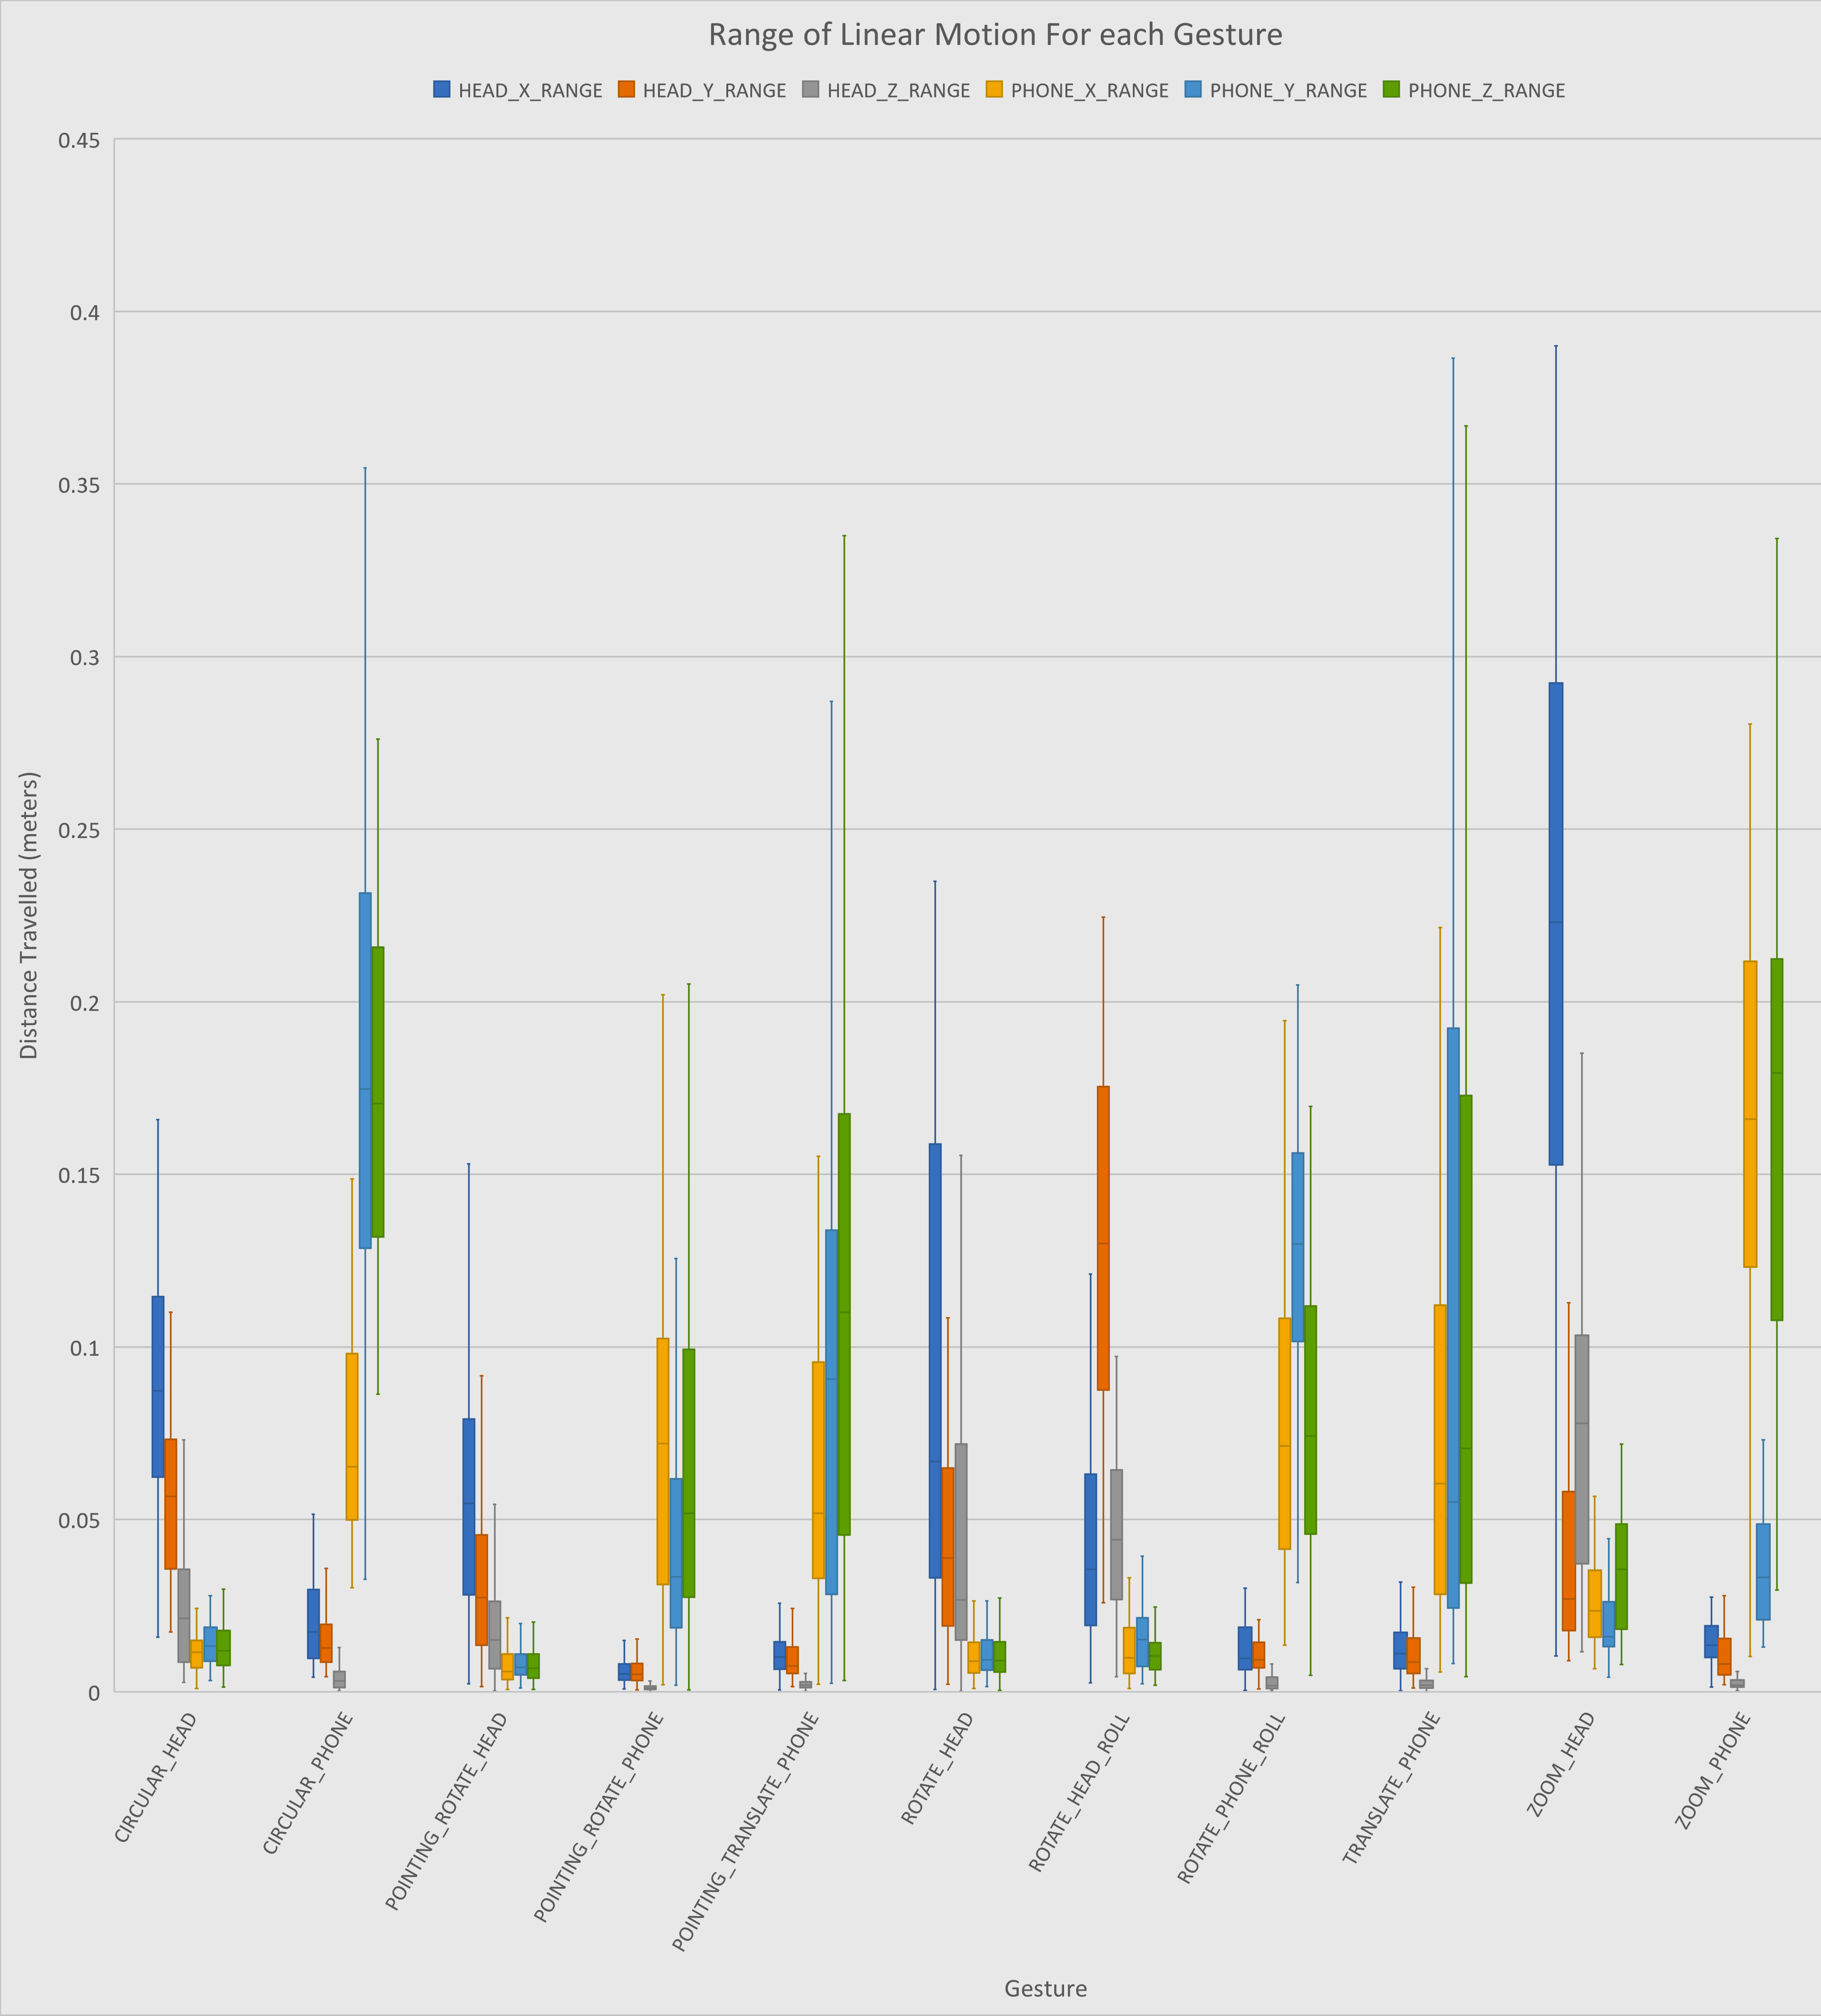
\includegraphics[width=\textwidth]{figures/RangeOfLinearMotion.png}
%     \caption{\label{fig:range_of_linear_motion} Range of linear motion for each gesture, in meters}
%     \Description{Box and Wisker plot showing the mean, min, max, and the first and third quartiles for the observed range of linear motion for each gesture recorded.}
% \end{figure}

\begin{figure}[H]
    \centering
    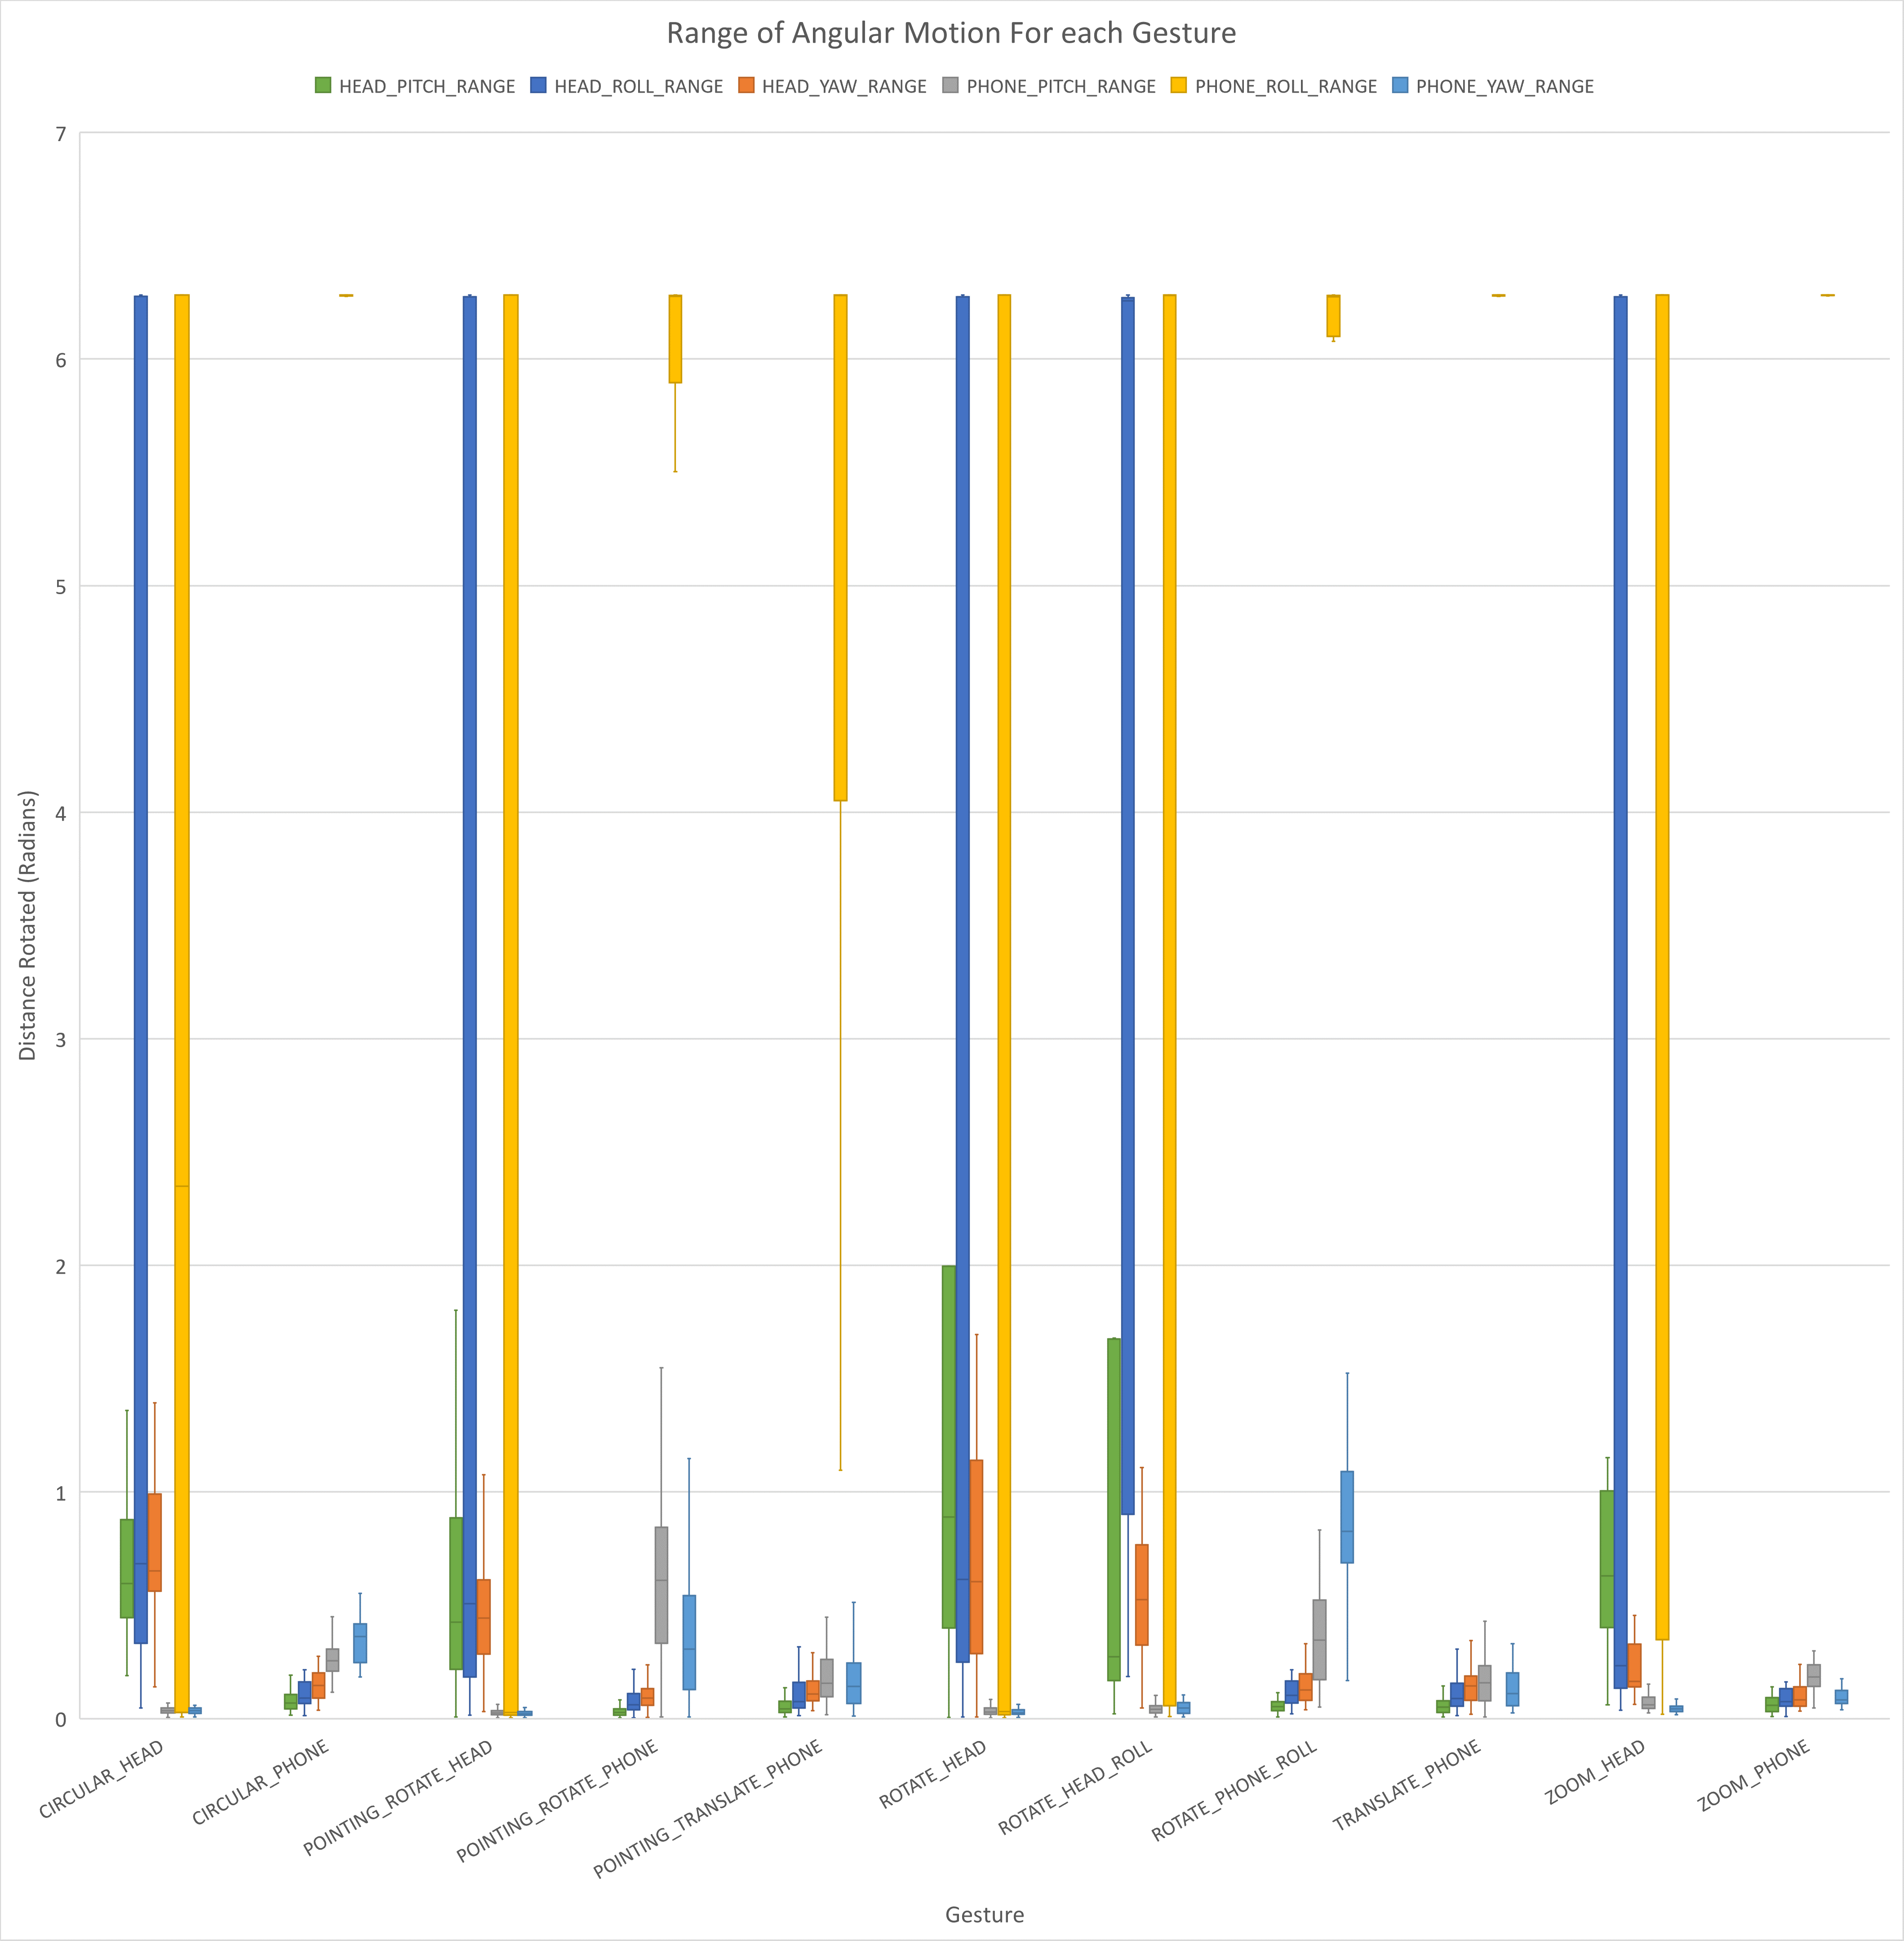
\includegraphics[width=\textwidth]{figures/RangeOfAngularMotion.png}
    \caption{\label{fig:range_of_angular_motion} Range of angular motion for each gesture, in meters}
    \Description{Box and Wisker plot showing the mean, min, max, and the first and third quartiles for the observed range of angular motion for each gesture recorded.}
\end{figure}

\newpage
\section{Code}
\subsection{Data Collection Application}
\url{https://github.com/whattheforkbomb/datacollection}

\subsection{Data Synchronisation}
\url{https://github.com/whattheforkbomb/dissertation_code/blob/trunk/datacollection/dataSynchronisation.py}

\subsection{YUV -> RGB Image Converter}
\url{https://github.com/whattheforkbomb/dissertation_code/blob/trunk/datacollection/imageGenerator.py}

\subsection{Data Resampling}
\url{https://github.com/whattheforkbomb/dissertation_code/blob/trunk/dataprocessing/data_analysis.ipynb}

\subsection{Model Development}
\url{https://github.com/whattheforkbomb/dissertation_code/blob/trunk/training/training.ipynb}

% Tell TexCount to start counting words again
%TC:endignore


\end{document}
\endinput